% Options for packages loaded elsewhere
\PassOptionsToPackage{unicode}{hyperref}
\PassOptionsToPackage{hyphens}{url}
\PassOptionsToPackage{dvipsnames,svgnames,x11names}{xcolor}
%
\documentclass[
  letterpaper,
  DIV=11,
  numbers=noendperiod]{scrartcl}

\usepackage{amsmath,amssymb}
\usepackage{iftex}
\ifPDFTeX
  \usepackage[T1]{fontenc}
  \usepackage[utf8]{inputenc}
  \usepackage{textcomp} % provide euro and other symbols
\else % if luatex or xetex
  \usepackage{unicode-math}
  \defaultfontfeatures{Scale=MatchLowercase}
  \defaultfontfeatures[\rmfamily]{Ligatures=TeX,Scale=1}
\fi
\usepackage{lmodern}
\ifPDFTeX\else  
    % xetex/luatex font selection
\fi
% Use upquote if available, for straight quotes in verbatim environments
\IfFileExists{upquote.sty}{\usepackage{upquote}}{}
\IfFileExists{microtype.sty}{% use microtype if available
  \usepackage[]{microtype}
  \UseMicrotypeSet[protrusion]{basicmath} % disable protrusion for tt fonts
}{}
\makeatletter
\@ifundefined{KOMAClassName}{% if non-KOMA class
  \IfFileExists{parskip.sty}{%
    \usepackage{parskip}
  }{% else
    \setlength{\parindent}{0pt}
    \setlength{\parskip}{6pt plus 2pt minus 1pt}}
}{% if KOMA class
  \KOMAoptions{parskip=half}}
\makeatother
\usepackage{xcolor}
\setlength{\emergencystretch}{3em} % prevent overfull lines
\setcounter{secnumdepth}{5}
% Make \paragraph and \subparagraph free-standing
\makeatletter
\ifx\paragraph\undefined\else
  \let\oldparagraph\paragraph
  \renewcommand{\paragraph}{
    \@ifstar
      \xxxParagraphStar
      \xxxParagraphNoStar
  }
  \newcommand{\xxxParagraphStar}[1]{\oldparagraph*{#1}\mbox{}}
  \newcommand{\xxxParagraphNoStar}[1]{\oldparagraph{#1}\mbox{}}
\fi
\ifx\subparagraph\undefined\else
  \let\oldsubparagraph\subparagraph
  \renewcommand{\subparagraph}{
    \@ifstar
      \xxxSubParagraphStar
      \xxxSubParagraphNoStar
  }
  \newcommand{\xxxSubParagraphStar}[1]{\oldsubparagraph*{#1}\mbox{}}
  \newcommand{\xxxSubParagraphNoStar}[1]{\oldsubparagraph{#1}\mbox{}}
\fi
\makeatother

\usepackage{color}
\usepackage{fancyvrb}
\newcommand{\VerbBar}{|}
\newcommand{\VERB}{\Verb[commandchars=\\\{\}]}
\DefineVerbatimEnvironment{Highlighting}{Verbatim}{commandchars=\\\{\}}
% Add ',fontsize=\small' for more characters per line
\usepackage{framed}
\definecolor{shadecolor}{RGB}{241,243,245}
\newenvironment{Shaded}{\begin{snugshade}}{\end{snugshade}}
\newcommand{\AlertTok}[1]{\textcolor[rgb]{0.68,0.00,0.00}{#1}}
\newcommand{\AnnotationTok}[1]{\textcolor[rgb]{0.37,0.37,0.37}{#1}}
\newcommand{\AttributeTok}[1]{\textcolor[rgb]{0.40,0.45,0.13}{#1}}
\newcommand{\BaseNTok}[1]{\textcolor[rgb]{0.68,0.00,0.00}{#1}}
\newcommand{\BuiltInTok}[1]{\textcolor[rgb]{0.00,0.23,0.31}{#1}}
\newcommand{\CharTok}[1]{\textcolor[rgb]{0.13,0.47,0.30}{#1}}
\newcommand{\CommentTok}[1]{\textcolor[rgb]{0.37,0.37,0.37}{#1}}
\newcommand{\CommentVarTok}[1]{\textcolor[rgb]{0.37,0.37,0.37}{\textit{#1}}}
\newcommand{\ConstantTok}[1]{\textcolor[rgb]{0.56,0.35,0.01}{#1}}
\newcommand{\ControlFlowTok}[1]{\textcolor[rgb]{0.00,0.23,0.31}{\textbf{#1}}}
\newcommand{\DataTypeTok}[1]{\textcolor[rgb]{0.68,0.00,0.00}{#1}}
\newcommand{\DecValTok}[1]{\textcolor[rgb]{0.68,0.00,0.00}{#1}}
\newcommand{\DocumentationTok}[1]{\textcolor[rgb]{0.37,0.37,0.37}{\textit{#1}}}
\newcommand{\ErrorTok}[1]{\textcolor[rgb]{0.68,0.00,0.00}{#1}}
\newcommand{\ExtensionTok}[1]{\textcolor[rgb]{0.00,0.23,0.31}{#1}}
\newcommand{\FloatTok}[1]{\textcolor[rgb]{0.68,0.00,0.00}{#1}}
\newcommand{\FunctionTok}[1]{\textcolor[rgb]{0.28,0.35,0.67}{#1}}
\newcommand{\ImportTok}[1]{\textcolor[rgb]{0.00,0.46,0.62}{#1}}
\newcommand{\InformationTok}[1]{\textcolor[rgb]{0.37,0.37,0.37}{#1}}
\newcommand{\KeywordTok}[1]{\textcolor[rgb]{0.00,0.23,0.31}{\textbf{#1}}}
\newcommand{\NormalTok}[1]{\textcolor[rgb]{0.00,0.23,0.31}{#1}}
\newcommand{\OperatorTok}[1]{\textcolor[rgb]{0.37,0.37,0.37}{#1}}
\newcommand{\OtherTok}[1]{\textcolor[rgb]{0.00,0.23,0.31}{#1}}
\newcommand{\PreprocessorTok}[1]{\textcolor[rgb]{0.68,0.00,0.00}{#1}}
\newcommand{\RegionMarkerTok}[1]{\textcolor[rgb]{0.00,0.23,0.31}{#1}}
\newcommand{\SpecialCharTok}[1]{\textcolor[rgb]{0.37,0.37,0.37}{#1}}
\newcommand{\SpecialStringTok}[1]{\textcolor[rgb]{0.13,0.47,0.30}{#1}}
\newcommand{\StringTok}[1]{\textcolor[rgb]{0.13,0.47,0.30}{#1}}
\newcommand{\VariableTok}[1]{\textcolor[rgb]{0.07,0.07,0.07}{#1}}
\newcommand{\VerbatimStringTok}[1]{\textcolor[rgb]{0.13,0.47,0.30}{#1}}
\newcommand{\WarningTok}[1]{\textcolor[rgb]{0.37,0.37,0.37}{\textit{#1}}}

\providecommand{\tightlist}{%
  \setlength{\itemsep}{0pt}\setlength{\parskip}{0pt}}\usepackage{longtable,booktabs,array}
\usepackage{calc} % for calculating minipage widths
% Correct order of tables after \paragraph or \subparagraph
\usepackage{etoolbox}
\makeatletter
\patchcmd\longtable{\par}{\if@noskipsec\mbox{}\fi\par}{}{}
\makeatother
% Allow footnotes in longtable head/foot
\IfFileExists{footnotehyper.sty}{\usepackage{footnotehyper}}{\usepackage{footnote}}
\makesavenoteenv{longtable}
\usepackage{graphicx}
\makeatletter
\newsavebox\pandoc@box
\newcommand*\pandocbounded[1]{% scales image to fit in text height/width
  \sbox\pandoc@box{#1}%
  \Gscale@div\@tempa{\textheight}{\dimexpr\ht\pandoc@box+\dp\pandoc@box\relax}%
  \Gscale@div\@tempb{\linewidth}{\wd\pandoc@box}%
  \ifdim\@tempb\p@<\@tempa\p@\let\@tempa\@tempb\fi% select the smaller of both
  \ifdim\@tempa\p@<\p@\scalebox{\@tempa}{\usebox\pandoc@box}%
  \else\usebox{\pandoc@box}%
  \fi%
}
% Set default figure placement to htbp
\def\fps@figure{htbp}
\makeatother

% load packages
\usepackage{geometry}
\usepackage{xcolor}
\usepackage{eso-pic}
\usepackage{fancyhdr}
\usepackage{sectsty}
\usepackage{fontspec}
\usepackage{titlesec}

%% Set page size with a wider right margin
\geometry{a4paper, total={170mm,257mm}, left=20mm, top=20mm, bottom=20mm, right=50mm}

%% Let's define some colours
\definecolor{light}{HTML}{E6E6FA}
\definecolor{highlight}{HTML}{800080}
\definecolor{dark}{HTML}{330033}

%% Let's add the border on the right hand side 
\AddToShipoutPicture{% 
    \AtPageLowerLeft{% 
        \put(\LenToUnit{\dimexpr\paperwidth-3cm},0){% 
            \color{light}\rule{3cm}{\LenToUnit\paperheight}%
          }%
     }%
     % logo
    \AtPageLowerLeft{% start the bar at the bottom right of the page
        \put(\LenToUnit{\dimexpr\paperwidth-2.25cm},27.2cm){% move it to the top right
            \color{light}
\includegraphics[width=1.5cm]{_extensions/nrennie/PrettyPDF/logo.png}
          }%
     }%
}

%% Style the page number
\fancypagestyle{mystyle}{
  \fancyhf{}
  \renewcommand\headrulewidth{0pt}
  \fancyfoot[R]{\thepage}
  \fancyfootoffset{3.5cm}
}
\setlength{\footskip}{20pt}

%% style the chapter/section fonts
\chapterfont{\color{dark}\fontsize{20}{16.8}\selectfont}
\sectionfont{\color{dark}\fontsize{20}{16.8}\selectfont}
\subsectionfont{\color{dark}\fontsize{14}{16.8}\selectfont}
\titleformat{\subsection}
  {\sffamily\Large\bfseries}{\thesection}{1em}{}[{\titlerule[0.8pt]}]
  
% left align title
\makeatletter
\renewcommand{\maketitle}{\bgroup\setlength{\parindent}{0pt}
\begin{flushleft}
  {\sffamily\huge\textbf{\MakeUppercase{\@title}}} \vspace{0.3cm} \newline
  {\Large {\@subtitle}} \newline
  \@author
\end{flushleft}\egroup
}
\makeatother

%% Use some custom fonts
\setsansfont{Ubuntu}[
    Path=_extensions/nrennie/PrettyPDF/Ubuntu/,
    Scale=0.9,
    Extension = .ttf,
    UprightFont=*-Regular,
    BoldFont=*-Bold,
    ItalicFont=*-Italic,
    ]

\setmainfont{Ubuntu}[
    Path=_extensions/nrennie/PrettyPDF/Ubuntu/,
    Scale=0.9,
    Extension = .ttf,
    UprightFont=*-Regular,
    BoldFont=*-Bold,
    ItalicFont=*-Italic,
    ]
\KOMAoption{captions}{tableheading}
\makeatletter
\@ifpackageloaded{tcolorbox}{}{\usepackage[skins,breakable]{tcolorbox}}
\@ifpackageloaded{fontawesome5}{}{\usepackage{fontawesome5}}
\definecolor{quarto-callout-color}{HTML}{909090}
\definecolor{quarto-callout-note-color}{HTML}{0758E5}
\definecolor{quarto-callout-important-color}{HTML}{CC1914}
\definecolor{quarto-callout-warning-color}{HTML}{EB9113}
\definecolor{quarto-callout-tip-color}{HTML}{00A047}
\definecolor{quarto-callout-caution-color}{HTML}{FC5300}
\definecolor{quarto-callout-color-frame}{HTML}{acacac}
\definecolor{quarto-callout-note-color-frame}{HTML}{4582ec}
\definecolor{quarto-callout-important-color-frame}{HTML}{d9534f}
\definecolor{quarto-callout-warning-color-frame}{HTML}{f0ad4e}
\definecolor{quarto-callout-tip-color-frame}{HTML}{02b875}
\definecolor{quarto-callout-caution-color-frame}{HTML}{fd7e14}
\makeatother
\makeatletter
\@ifpackageloaded{caption}{}{\usepackage{caption}}
\AtBeginDocument{%
\ifdefined\contentsname
  \renewcommand*\contentsname{Table of contents}
\else
  \newcommand\contentsname{Table of contents}
\fi
\ifdefined\listfigurename
  \renewcommand*\listfigurename{List of Figures}
\else
  \newcommand\listfigurename{List of Figures}
\fi
\ifdefined\listtablename
  \renewcommand*\listtablename{List of Tables}
\else
  \newcommand\listtablename{List of Tables}
\fi
\ifdefined\figurename
  \renewcommand*\figurename{Figure}
\else
  \newcommand\figurename{Figure}
\fi
\ifdefined\tablename
  \renewcommand*\tablename{Table}
\else
  \newcommand\tablename{Table}
\fi
}
\@ifpackageloaded{float}{}{\usepackage{float}}
\floatstyle{ruled}
\@ifundefined{c@chapter}{\newfloat{codelisting}{h}{lop}}{\newfloat{codelisting}{h}{lop}[chapter]}
\floatname{codelisting}{Listing}
\newcommand*\listoflistings{\listof{codelisting}{List of Listings}}
\makeatother
\makeatletter
\makeatother
\makeatletter
\@ifpackageloaded{caption}{}{\usepackage{caption}}
\@ifpackageloaded{subcaption}{}{\usepackage{subcaption}}
\makeatother
\makeatletter
\@ifpackageloaded{tcolorbox}{}{\usepackage[skins,breakable]{tcolorbox}}
\makeatother
\makeatletter
\@ifundefined{shadecolor}{\definecolor{shadecolor}{rgb}{.97, .97, .97}}{}
\makeatother
\makeatletter
\@ifundefined{codebgcolor}{\definecolor{codebgcolor}{named}{light}}{}
\makeatother
\makeatletter
\ifdefined\Shaded\renewenvironment{Shaded}{\begin{tcolorbox}[colback={codebgcolor}, boxrule=0pt, enhanced, frame hidden, sharp corners, breakable]}{\end{tcolorbox}}\fi
\makeatother

\usepackage{bookmark}

\IfFileExists{xurl.sty}{\usepackage{xurl}}{} % add URL line breaks if available
\urlstyle{same} % disable monospaced font for URLs
\hypersetup{
  pdftitle={Practical 5},
  colorlinks=true,
  linkcolor={highlight},
  filecolor={Maroon},
  citecolor={Blue},
  urlcolor={highlight},
  pdfcreator={LaTeX via pandoc}}


\title{Practical 5}
\author{}
\date{}

\begin{document}
\maketitle

\pagestyle{mystyle}


\textbf{Aim of this practical:}

In this first practical we are going to fit spatial modes for Areal,
Geostatistical and Point-Process Data.

\section{Models for areal data}\label{models-for-areal-data}

In this practical we are going to fit an areal model. We will:

\begin{itemize}
\item
  Learn how to fit an areal model in \texttt{inlabru}
\item
  Learn how to add spatial covariates to the model
\item
  Learn how to do predictions
\item
  Learn how to simulate from the fitted model
\end{itemize}

\begin{center}\rule{0.5\linewidth}{0.5pt}\end{center}

Libraries to load:

\begin{Shaded}
\begin{Highlighting}[]
\FunctionTok{library}\NormalTok{(dplyr)}
\FunctionTok{library}\NormalTok{(INLA)}
\FunctionTok{library}\NormalTok{(ggplot2)}
\FunctionTok{library}\NormalTok{(patchwork)}
\FunctionTok{library}\NormalTok{(inlabru)   }
\FunctionTok{library}\NormalTok{(mapview)}

\CommentTok{\# load some libraries to generate nice map plots}
\FunctionTok{library}\NormalTok{(scico)}
\end{Highlighting}
\end{Shaded}

\subsection{The data}\label{the-data}

We consider data on respiratory hospitalizations for Greater Glasgow and
Clyde in 2007. The data are available from the \texttt{CARBayesdata} R
Package:

\begin{Shaded}
\begin{Highlighting}[]
\FunctionTok{library}\NormalTok{(CARBayesdata)}

\FunctionTok{data}\NormalTok{(pollutionhealthdata)}
\FunctionTok{data}\NormalTok{(GGHB.IZ)}
\end{Highlighting}
\end{Shaded}

The \texttt{pollutionhealthdata} contains the spatiotemporal data on
respiratory hospitalizations, air pollution concentrations and
socio-economic deprivation covariates for the 271 Intermediate Zones
(IZ) that make up the Greater Glasgow and Clyde health board in
Scotland. Data are provided by the
\href{http://statistics.gov.scot.}{Scottish Government} and the
available variables are:

\begin{itemize}
\tightlist
\item
  \texttt{IZ}: unique identifier for each IZ.
\item
  \texttt{year}: the year when the measurements were taken
\item
  \texttt{observed}: observed numbers of hospitalizations due to
  respiratory disease.
\item
  \texttt{expected}: expected numbers of hospitalizations due to
  respiratory disease computed using indirect standardisation from
  Scotland-wide respiratory hospitalization rates.
\item
  \texttt{pm10}: Average particulate matter (less than 10 microns)
  concentrations.
\item
  \texttt{jsa}: The percentage of working age people who are in receipt
  of Job Seekers Allowance
\item
  \texttt{price}: Average property price (divided by 100,000).
\end{itemize}

The \texttt{GGHB.IZ} data is a Simple Features (\texttt{sf}) object
containing the spatial polygon information for the set of 271
Intermediate Zones (IZ), that make up of the Greater Glasgow and Clyde
health board in Scotland ( Figure~\ref{fig-GGC} ).

\begin{figure}

\centering{

\pandocbounded{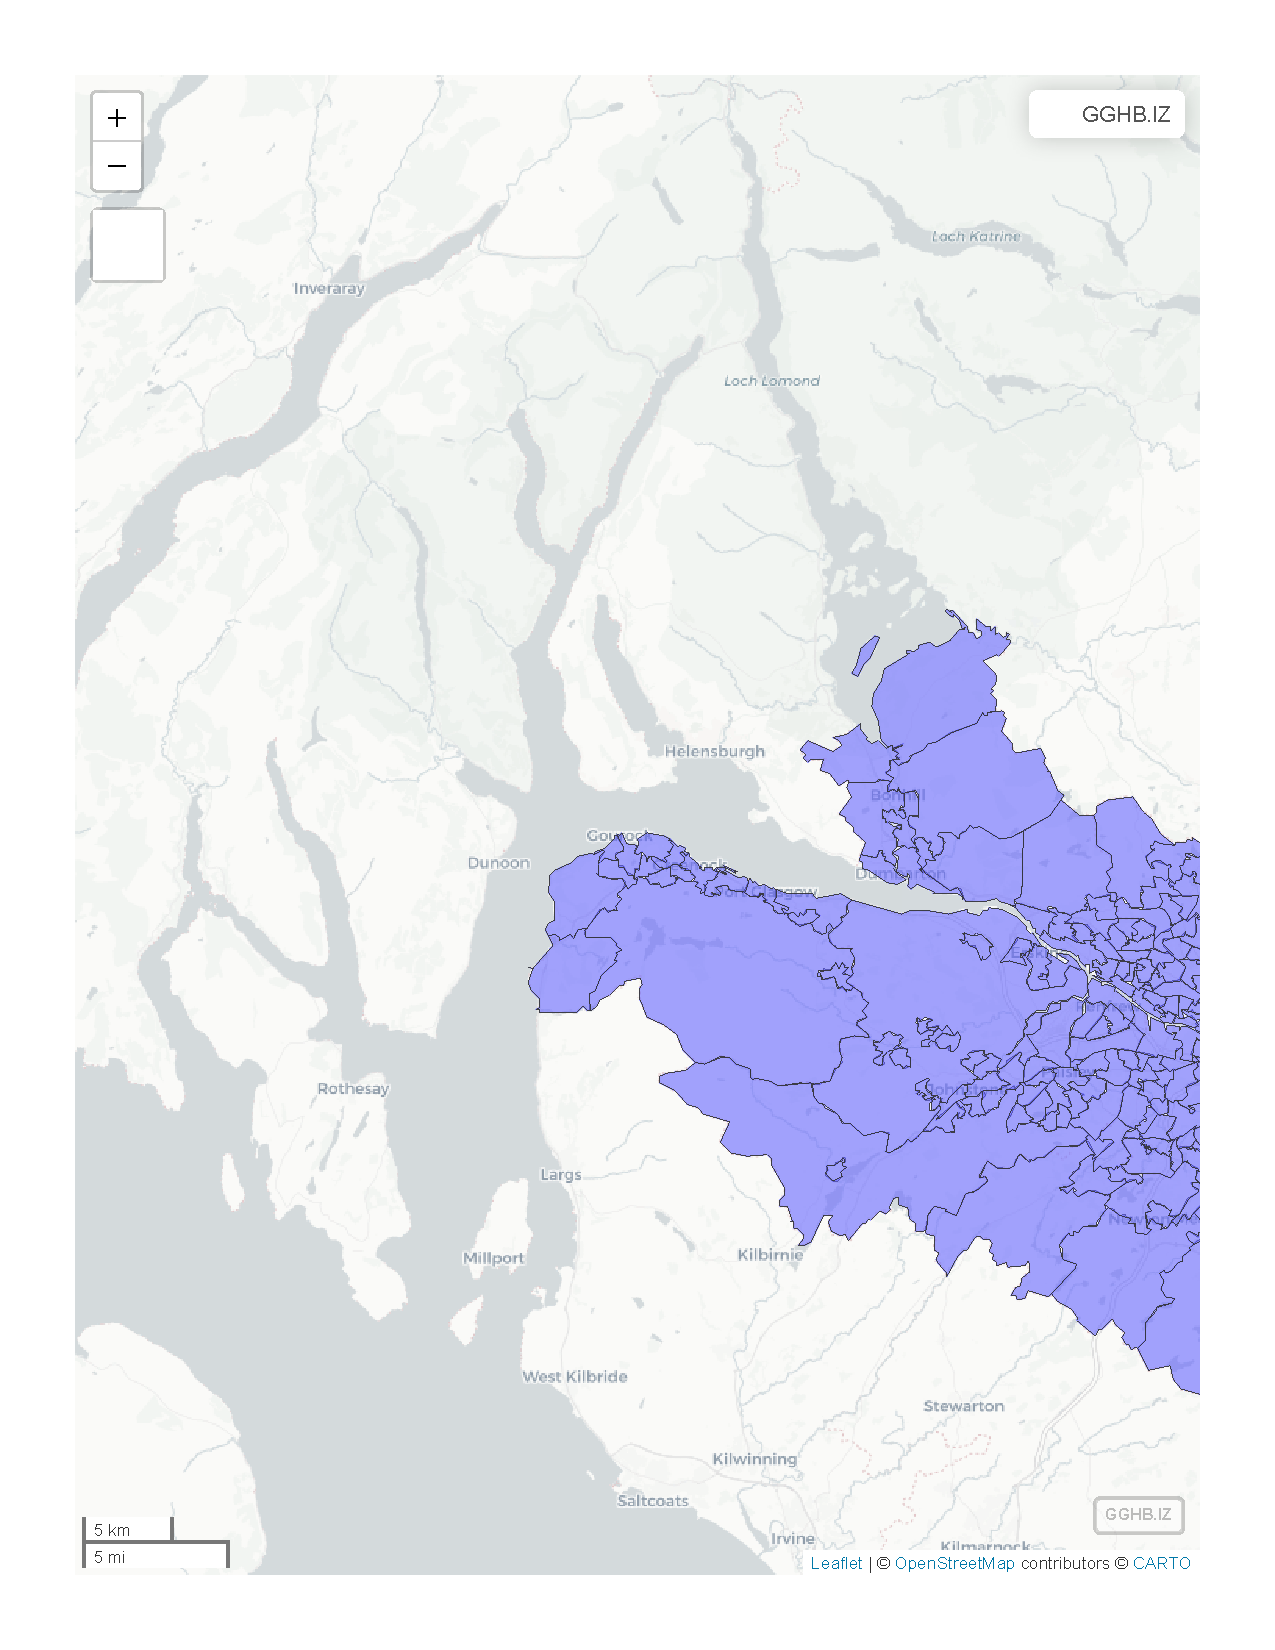
\includegraphics[keepaspectratio]{day3_practical_5_files/figure-pdf/fig-GGC-1.pdf}}

}

\caption{\label{fig-GGC}Greater Glasgow and Clyde health board
represented by 271 Intermediate Zones}

\end{figure}%

We first merge the two dataset and select only one year of data, compute
the SME and plot the observed

\begin{Shaded}
\begin{Highlighting}[]
\NormalTok{resp\_cases }\OtherTok{\textless{}{-}} \FunctionTok{merge}\NormalTok{(GGHB.IZ }\SpecialCharTok{\%\textgreater{}\%}
                      \FunctionTok{mutate}\NormalTok{(}\AttributeTok{space =} \DecValTok{1}\SpecialCharTok{:}\FunctionTok{dim}\NormalTok{(GGHB.IZ)[}\DecValTok{1}\NormalTok{]),}
\NormalTok{                             pollutionhealthdata, }\AttributeTok{by =} \StringTok{"IZ"}\NormalTok{) }\SpecialCharTok{\%\textgreater{}\%}
  \FunctionTok{filter}\NormalTok{(year }\SpecialCharTok{==} \DecValTok{2007}\NormalTok{) }\SpecialCharTok{\%\textgreater{}\%}
    \FunctionTok{mutate}\NormalTok{(}\AttributeTok{SMR =}\NormalTok{ observed}\SpecialCharTok{/}\NormalTok{expected)}

\FunctionTok{ggplot}\NormalTok{() }\SpecialCharTok{+} \FunctionTok{geom\_sf}\NormalTok{(}\AttributeTok{data =}\NormalTok{ resp\_cases, }\FunctionTok{aes}\NormalTok{(}\AttributeTok{fill =}\NormalTok{ SMR)) }\SpecialCharTok{+} \FunctionTok{scale\_fill\_scico}\NormalTok{(}\AttributeTok{direction =} \SpecialCharTok{{-}}\DecValTok{1}\NormalTok{)}
\end{Highlighting}
\end{Shaded}

\pandocbounded{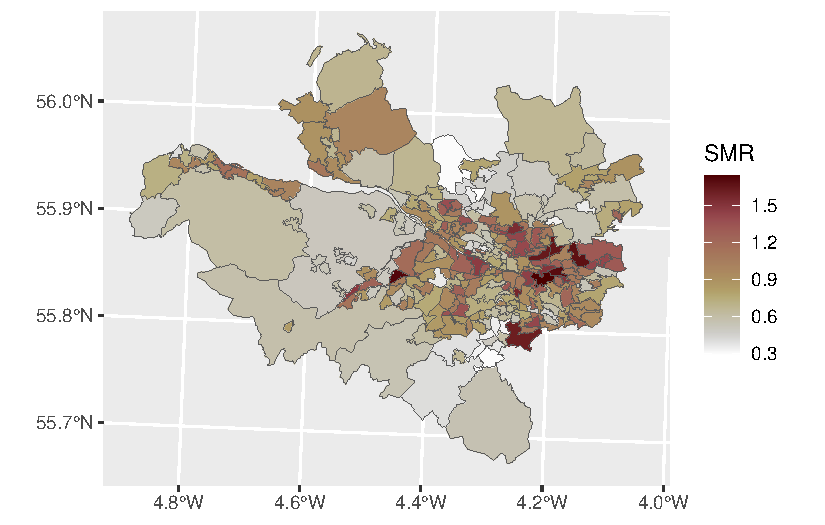
\includegraphics[keepaspectratio]{day3_practical_5_files/figure-pdf/unnamed-chunk-5-1.pdf}}

Then we compute the adjacency matrix using the functions
\texttt{poly2nb()} and \texttt{nb2mat()} in the \texttt{spdep} library.
We then convert the adjacency matrix into the precision matrix
\(\mathbf{Q}\) of the CAR model. Remember this matrix has, on the
diagonal the number of e

\begin{Shaded}
\begin{Highlighting}[]
\FunctionTok{library}\NormalTok{(spdep)}

\NormalTok{W.nb }\OtherTok{\textless{}{-}} \FunctionTok{poly2nb}\NormalTok{(GGHB.IZ,}\AttributeTok{queen =} \ConstantTok{TRUE}\NormalTok{)}
\NormalTok{R }\OtherTok{\textless{}{-}} \FunctionTok{nb2mat}\NormalTok{(W.nb, }\AttributeTok{style =} \StringTok{"B"}\NormalTok{, }\AttributeTok{zero.policy =} \ConstantTok{TRUE}\NormalTok{)}

\NormalTok{diag }\OtherTok{=} \FunctionTok{apply}\NormalTok{(R,}\DecValTok{1}\NormalTok{,sum)}
\NormalTok{Q }\OtherTok{=} \SpecialCharTok{{-}}\NormalTok{R}
\FunctionTok{diag}\NormalTok{(Q) }\OtherTok{=}\NormalTok{ diag}
\end{Highlighting}
\end{Shaded}

\subsection{The model}\label{the-model}

We fit a first model to the data where we consider a Poisson model for
the observed cases.

\textbf{Stage 1} Model for the response \[
y_i|\eta_i\sim\text{Poisson}(E_i\lambda_i)
\] where \(E_i\) are the expected cases for area \(i\).

\textbf{Stage 2} Latent field model \[
\eta_i = \text{log}(\lambda_i) = \beta_0 + \omega_i + z_i
\] where

\begin{itemize}
\tightlist
\item
  \(\beta_0\) is a common intercept
\item
  \(\mathbf{\omega} = (\omega_1, \dots, \omega_k)\) is a conditional
  Autorgressive model (CAR) with precision matrix \(\tau_1\mathbf{Q}\)
\item
  \(\mathbf{z} = (z_1, \dots, z_k)\) is an unstrictured random effect
  with precision \(\tau_2\)
\end{itemize}

\textbf{Stage 3} Hyperparameters

The hyperparameters of the model are \(\tau_1\) and \(\tau_2\)

\textbf{NOTE} In this case the linear predictor \(\eta\) consists of
three components!!

\begin{tcolorbox}[enhanced jigsaw, coltitle=black, bottomtitle=1mm, leftrule=.75mm, left=2mm, colback=white, colbacktitle=quarto-callout-warning-color!10!white, breakable, toptitle=1mm, titlerule=0mm, title={Task}, arc=.35mm, toprule=.15mm, bottomrule=.15mm, rightrule=.15mm, opacitybacktitle=0.6, opacityback=0, colframe=quarto-callout-warning-color-frame]

Fit the above model in using \texttt{inlabru} by completing the
following code:

\begin{Shaded}
\begin{Highlighting}[]
\NormalTok{cmp }\OtherTok{=} \ErrorTok{\textasciitilde{}} \FunctionTok{Intercept}\NormalTok{(}\DecValTok{1}\NormalTok{) }\SpecialCharTok{+} \FunctionTok{space}\NormalTok{(...) }\SpecialCharTok{+} \FunctionTok{iid}\NormalTok{(...)}

\NormalTok{formula }\OtherTok{=}\NormalTok{ ...}


\NormalTok{lik }\OtherTok{=} \FunctionTok{bru\_obs}\NormalTok{(}\AttributeTok{formula =}\NormalTok{ formula, }
              \AttributeTok{family =}\NormalTok{ ...,}
              \AttributeTok{E =}\NormalTok{ ...,}
              \AttributeTok{data =}\NormalTok{ ...)}

\NormalTok{fit }\OtherTok{=} \FunctionTok{bru}\NormalTok{(cmp, lik)}
\end{Highlighting}
\end{Shaded}

Answer

\begin{Shaded}
\begin{Highlighting}[]
\NormalTok{cmp }\OtherTok{=} \ErrorTok{\textasciitilde{}} \FunctionTok{Intercept}\NormalTok{(}\DecValTok{1}\NormalTok{) }\SpecialCharTok{+} \FunctionTok{space}\NormalTok{(space, }\AttributeTok{model =} \StringTok{"besag"}\NormalTok{, }\AttributeTok{graph =}\NormalTok{ Q) }\SpecialCharTok{+} \FunctionTok{iid}\NormalTok{(space, }\AttributeTok{model =} \StringTok{"iid"}\NormalTok{)}

\NormalTok{formula }\OtherTok{=}\NormalTok{ observed }\SpecialCharTok{\textasciitilde{}}\NormalTok{ Intercept }\SpecialCharTok{+}\NormalTok{ space }\SpecialCharTok{+}\NormalTok{ iid}

\NormalTok{lik }\OtherTok{=} \FunctionTok{bru\_obs}\NormalTok{(}\AttributeTok{formula =}\NormalTok{ formula, }
              \AttributeTok{family =} \StringTok{"poisson"}\NormalTok{,}
              \AttributeTok{E =}\NormalTok{ expected,}
              \AttributeTok{data =}\NormalTok{ resp\_cases)}

\NormalTok{fit }\OtherTok{=} \FunctionTok{bru}\NormalTok{(cmp, lik)}
\end{Highlighting}
\end{Shaded}

\end{tcolorbox}

After fitting the model we want to extract results.

\begin{tcolorbox}[enhanced jigsaw, coltitle=black, bottomtitle=1mm, leftrule=.75mm, left=2mm, colback=white, colbacktitle=quarto-callout-tip-color!10!white, breakable, toptitle=1mm, titlerule=0mm, title={Question}, arc=.35mm, toprule=.15mm, bottomrule=.15mm, rightrule=.15mm, opacitybacktitle=0.6, opacityback=0, colframe=quarto-callout-tip-color-frame]

\begin{enumerate}
\def\labelenumi{\arabic{enumi}.}
\item
  What is the estimated value for \(\beta_0\)?
  \_\_\_\_\_\_\_\_\_\_\_\_\_\_\_\_\_\_
\item
  Look at the estimated values of the hyperparameters using
  \texttt{fit\$summary.hyperpar} , which of the two spatial components
  (structured or unstructured) explains more of the variability in the
  counts?
\end{enumerate}

\begin{itemize}
\tightlist
\item
  \begin{enumerate}
  \def\labelenumi{(\Alph{enumi})}
  \tightlist
  \item
    structured\\
  \end{enumerate}
\item
  \begin{enumerate}
  \def\labelenumi{(\Alph{enumi})}
  \setcounter{enumi}{1}
  \tightlist
  \item
    unstructured
  \end{enumerate}
\end{itemize}

\end{tcolorbox}

We now look at the predictions over space.

\begin{tcolorbox}[enhanced jigsaw, coltitle=black, bottomtitle=1mm, leftrule=.75mm, left=2mm, colback=white, colbacktitle=quarto-callout-warning-color!10!white, breakable, toptitle=1mm, titlerule=0mm, title={Task}, arc=.35mm, toprule=.15mm, bottomrule=.15mm, rightrule=.15mm, opacitybacktitle=0.6, opacityback=0, colframe=quarto-callout-warning-color-frame]

Complete the code below to produce prediction of the linear predictor
\(\eta_i\) and of the risk \(\lambda_i\) and of the expected cases
\(E_i\exp(\lambda_i)\) over the whole space of interest. Then plot the
mean and sd of the resulting surfaces.

\begin{Shaded}
\begin{Highlighting}[]
\NormalTok{pred }\OtherTok{=} \FunctionTok{predict}\NormalTok{(fit, resp\_cases, }\SpecialCharTok{\textasciitilde{}}\FunctionTok{data.frame}\NormalTok{(}\AttributeTok{log\_risk =}\NormalTok{ ...,}
                                             \AttributeTok{risk =} \FunctionTok{exp}\NormalTok{(...),}
                                             \AttributeTok{cases =}\NormalTok{ ...}
\NormalTok{                                             ),}
               \AttributeTok{n.samples =} \DecValTok{1000}\NormalTok{)}
\end{Highlighting}
\end{Shaded}

Show Answer

\begin{Shaded}
\begin{Highlighting}[]
\CommentTok{\# produce predictions}
\NormalTok{pred }\OtherTok{=} \FunctionTok{predict}\NormalTok{(fit, resp\_cases, }\SpecialCharTok{\textasciitilde{}}\FunctionTok{data.frame}\NormalTok{(}\AttributeTok{log\_risk =}\NormalTok{ Intercept }\SpecialCharTok{+}\NormalTok{ space,}
                                             \AttributeTok{risk =} \FunctionTok{exp}\NormalTok{(Intercept }\SpecialCharTok{+}\NormalTok{ space),}
                                             \AttributeTok{cases =}\NormalTok{ expected }\SpecialCharTok{*} \FunctionTok{exp}\NormalTok{(Intercept }\SpecialCharTok{+}\NormalTok{ space)}
\NormalTok{                                             ),}
               \AttributeTok{n.samples =} \DecValTok{1000}\NormalTok{)}
\CommentTok{\# plot the predictions}

\NormalTok{p1 }\OtherTok{=} \FunctionTok{ggplot}\NormalTok{() }\SpecialCharTok{+} \FunctionTok{geom\_sf}\NormalTok{(}\AttributeTok{data =}\NormalTok{ pred}\SpecialCharTok{$}\NormalTok{log\_risk, }\FunctionTok{aes}\NormalTok{(}\AttributeTok{fill =}\NormalTok{ mean)) }\SpecialCharTok{+} \FunctionTok{scale\_fill\_scico}\NormalTok{(}\AttributeTok{direction =} \SpecialCharTok{{-}}\DecValTok{1}\NormalTok{) }\SpecialCharTok{+} \FunctionTok{ggtitle}\NormalTok{(}\StringTok{"mean log risk"}\NormalTok{)}
\NormalTok{p2 }\OtherTok{=} \FunctionTok{ggplot}\NormalTok{() }\SpecialCharTok{+} \FunctionTok{geom\_sf}\NormalTok{(}\AttributeTok{data =}\NormalTok{ pred}\SpecialCharTok{$}\NormalTok{log\_risk, }\FunctionTok{aes}\NormalTok{(}\AttributeTok{fill =}\NormalTok{ sd)) }\SpecialCharTok{+} \FunctionTok{scale\_fill\_scico}\NormalTok{(}\AttributeTok{direction =} \SpecialCharTok{{-}}\DecValTok{1}\NormalTok{) }\SpecialCharTok{+} \FunctionTok{ggtitle}\NormalTok{(}\StringTok{"sd log risk"}\NormalTok{)}
\NormalTok{p1 }\SpecialCharTok{+}\NormalTok{ p2}
\end{Highlighting}
\end{Shaded}

\pandocbounded{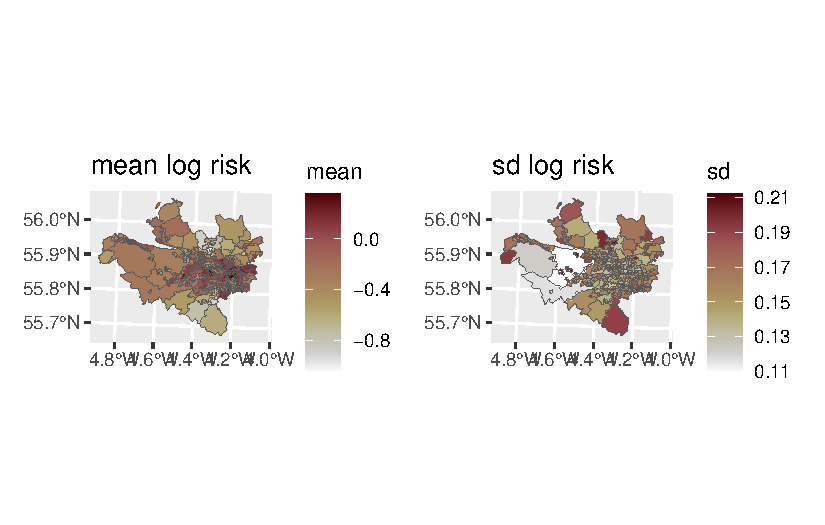
\includegraphics[keepaspectratio]{day3_practical_5_files/figure-pdf/unnamed-chunk-10-1.pdf}}

\begin{Shaded}
\begin{Highlighting}[]
\NormalTok{p1 }\OtherTok{=} \FunctionTok{ggplot}\NormalTok{() }\SpecialCharTok{+} \FunctionTok{geom\_sf}\NormalTok{(}\AttributeTok{data =}\NormalTok{ pred}\SpecialCharTok{$}\NormalTok{risk, }\FunctionTok{aes}\NormalTok{(}\AttributeTok{fill =}\NormalTok{ mean)) }\SpecialCharTok{+} \FunctionTok{scale\_fill\_scico}\NormalTok{(}\AttributeTok{direction =} \SpecialCharTok{{-}}\DecValTok{1}\NormalTok{) }\SpecialCharTok{+} \FunctionTok{ggtitle}\NormalTok{(}\StringTok{"mean  risk"}\NormalTok{)}
\NormalTok{p2 }\OtherTok{=} \FunctionTok{ggplot}\NormalTok{() }\SpecialCharTok{+} \FunctionTok{geom\_sf}\NormalTok{(}\AttributeTok{data =}\NormalTok{ pred}\SpecialCharTok{$}\NormalTok{risk, }\FunctionTok{aes}\NormalTok{(}\AttributeTok{fill =}\NormalTok{ sd)) }\SpecialCharTok{+} \FunctionTok{scale\_fill\_scico}\NormalTok{(}\AttributeTok{direction =} \SpecialCharTok{{-}}\DecValTok{1}\NormalTok{) }\SpecialCharTok{+} \FunctionTok{ggtitle}\NormalTok{(}\StringTok{"sd  risk"}\NormalTok{)}
\NormalTok{p1 }\SpecialCharTok{+}\NormalTok{ p2}
\end{Highlighting}
\end{Shaded}

\pandocbounded{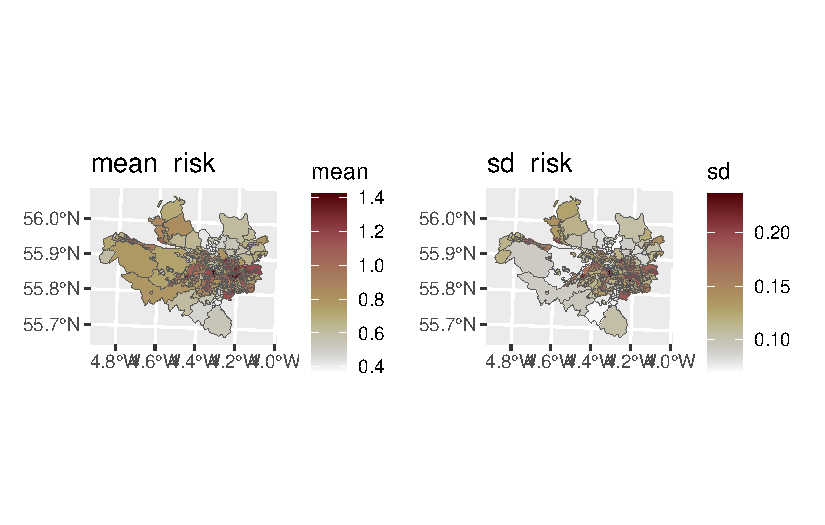
\includegraphics[keepaspectratio]{day3_practical_5_files/figure-pdf/unnamed-chunk-10-2.pdf}}

\begin{Shaded}
\begin{Highlighting}[]
\NormalTok{p1 }\OtherTok{=} \FunctionTok{ggplot}\NormalTok{() }\SpecialCharTok{+} \FunctionTok{geom\_sf}\NormalTok{(}\AttributeTok{data =}\NormalTok{ pred}\SpecialCharTok{$}\NormalTok{cases, }\FunctionTok{aes}\NormalTok{(}\AttributeTok{fill =}\NormalTok{ mean)) }\SpecialCharTok{+} \FunctionTok{scale\_fill\_scico}\NormalTok{(}\AttributeTok{direction =} \SpecialCharTok{{-}}\DecValTok{1}\NormalTok{)}\SpecialCharTok{+} \FunctionTok{ggtitle}\NormalTok{(}\StringTok{"mean  expected counts"}\NormalTok{)}
\NormalTok{p2 }\OtherTok{=} \FunctionTok{ggplot}\NormalTok{() }\SpecialCharTok{+} \FunctionTok{geom\_sf}\NormalTok{(}\AttributeTok{data =}\NormalTok{ pred}\SpecialCharTok{$}\NormalTok{cases, }\FunctionTok{aes}\NormalTok{(}\AttributeTok{fill =}\NormalTok{ sd)) }\SpecialCharTok{+} \FunctionTok{scale\_fill\_scico}\NormalTok{(}\AttributeTok{direction =} \SpecialCharTok{{-}}\DecValTok{1}\NormalTok{)}\SpecialCharTok{+} \FunctionTok{ggtitle}\NormalTok{(}\StringTok{"sd  expected counts"}\NormalTok{)}
\NormalTok{p1 }\SpecialCharTok{+}\NormalTok{ p2}
\end{Highlighting}
\end{Shaded}

\pandocbounded{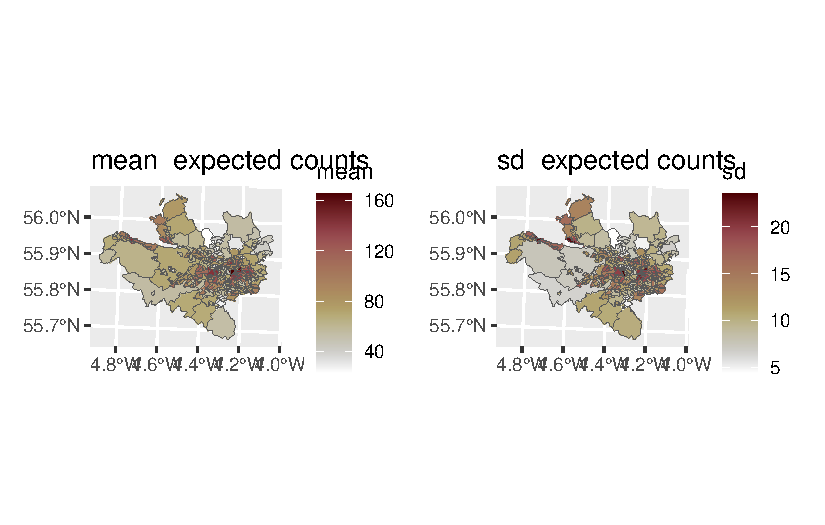
\includegraphics[keepaspectratio]{day3_practical_5_files/figure-pdf/unnamed-chunk-10-3.pdf}}

\end{tcolorbox}

Finally we want to compare our observations \(y_i\) with the predicted
means of the Poisson distribution \(E_i\exp(\lambda_i)\)

\begin{Shaded}
\begin{Highlighting}[]
\NormalTok{pred}\SpecialCharTok{$}\NormalTok{cases }\SpecialCharTok{\%\textgreater{}\%} \FunctionTok{ggplot}\NormalTok{() }\SpecialCharTok{+} \FunctionTok{geom\_point}\NormalTok{(}\FunctionTok{aes}\NormalTok{(observed, mean)) }\SpecialCharTok{+} 
  \FunctionTok{geom\_errorbar}\NormalTok{(}\FunctionTok{aes}\NormalTok{(observed, }\AttributeTok{ymin =}\NormalTok{ q0}\FloatTok{.025}\NormalTok{, }\AttributeTok{ymax =}\NormalTok{ q0}\FloatTok{.975}\NormalTok{)) }\SpecialCharTok{+}
  \FunctionTok{geom\_abline}\NormalTok{(}\AttributeTok{intercept =} \DecValTok{0}\NormalTok{, }\AttributeTok{slope =} \DecValTok{1}\NormalTok{)}
\end{Highlighting}
\end{Shaded}

\pandocbounded{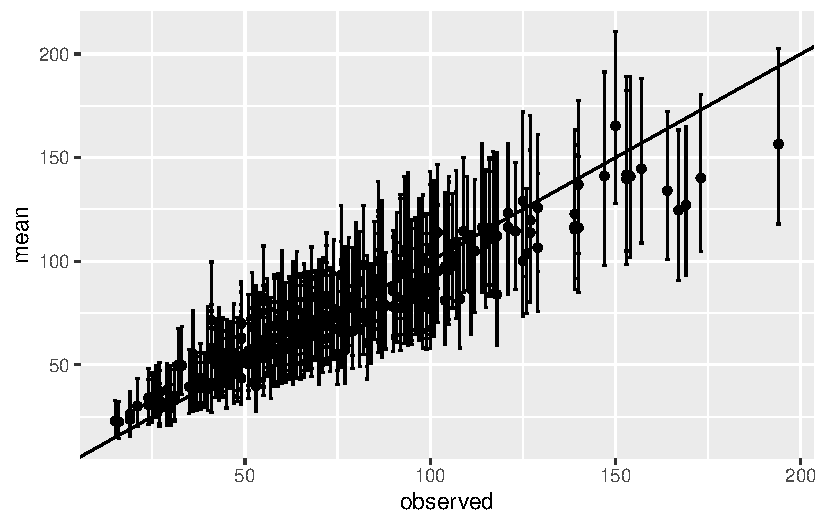
\includegraphics[keepaspectratio]{day3_practical_5_files/figure-pdf/unnamed-chunk-11-1.pdf}}

\textbf{Note:} Here we are predicting the \emph{mean} of counts, not the
counts!!! Predicting counts is the theme of the next task!

\subsection{Getting prediction
densities}\label{getting-prediction-densities}

Posterior predictive distributions, that is
\(\pi(y_i^{\text{new}}|\mathbf{y})\) are of interest in many applied
problems. The \texttt{bru()} function does not return predictive
densities. In the previous step we have computed predictions for the
\texttt{expected\ counts} \(\pi(E_i\lambda_i|\mathbf{y})\). The
predictive distribution is then: \[
\pi(y_i^{\text{new}}|\mathbf{y}) = \int \pi(y_i|E_i\lambda_i)\pi(E_i\lambda_i|\mathbf{y})\ dE_i\lambda_i
\] where, in our case, \(\pi(y_i|E_i\lambda_i)\) is Poisson with mean
\(E_i\lambda_i\). We can achieve this using the following algorith:

\begin{enumerate}
\def\labelenumi{\arabic{enumi}.}
\tightlist
\item
  Simulate \(n\) replicates of \(g^k = E_i\lambda_i\) for
  \(k = 1,\dots,n\) using the function \emph{generate()} which takes the
  same input as \emph{predict()}
\item
  For each of the \(k\) replicates simulate a new value \(y_i^{new}\)
  using the function \emph{rpois()}
\item
  Summarise the \(n\) samples of \(y_i^{new}\) using, for example the
  mean and the 0.025 and 0.975 quantiles.
\end{enumerate}

Here is the code:

\begin{Shaded}
\begin{Highlighting}[]
\CommentTok{\# simulate 1000 realizations of E\_i\textbackslash{}lambda\_i}
\NormalTok{expected\_counts }\OtherTok{=} \FunctionTok{generate}\NormalTok{(fit, resp\_cases, }
                           \SpecialCharTok{\textasciitilde{}}\NormalTok{ expected }\SpecialCharTok{*} \FunctionTok{exp}\NormalTok{(Intercept }\SpecialCharTok{+}\NormalTok{ space),}
                           \AttributeTok{n.samples =} \DecValTok{1000}\NormalTok{)}


\CommentTok{\# simulate poisson data}
\NormalTok{aa }\OtherTok{=} \FunctionTok{rpois}\NormalTok{(}\DecValTok{271}\SpecialCharTok{*}\DecValTok{1000}\NormalTok{, }\AttributeTok{lambda =} \FunctionTok{as.vector}\NormalTok{(expected\_counts))}
\NormalTok{sim\_counts }\OtherTok{=} \FunctionTok{matrix}\NormalTok{(aa, }\DecValTok{271}\NormalTok{, }\DecValTok{1000}\NormalTok{)}

\CommentTok{\# summarise the samples with posterior means and quantiles}
\NormalTok{pred\_counts }\OtherTok{=} \FunctionTok{data.frame}\NormalTok{(}\AttributeTok{observed =}\NormalTok{ resp\_cases}\SpecialCharTok{$}\NormalTok{observed,}
                         \AttributeTok{m =} \FunctionTok{apply}\NormalTok{(sim\_counts,}\DecValTok{1}\NormalTok{,mean),}
                         \AttributeTok{q1 =} \FunctionTok{apply}\NormalTok{(sim\_counts,}\DecValTok{1}\NormalTok{,quantile, }\FloatTok{0.025}\NormalTok{),}
                         \AttributeTok{q2 =} \FunctionTok{apply}\NormalTok{(sim\_counts,}\DecValTok{1}\NormalTok{,quantile, }\FloatTok{0.975}\NormalTok{),}
                         \AttributeTok{vv =} \FunctionTok{apply}\NormalTok{(sim\_counts,}\DecValTok{1}\NormalTok{,var)}
\NormalTok{                         )}
\end{Highlighting}
\end{Shaded}

\begin{tcolorbox}[enhanced jigsaw, coltitle=black, bottomtitle=1mm, leftrule=.75mm, left=2mm, colback=white, colbacktitle=quarto-callout-warning-color!10!white, breakable, toptitle=1mm, titlerule=0mm, title={Task}, arc=.35mm, toprule=.15mm, bottomrule=.15mm, rightrule=.15mm, opacitybacktitle=0.6, opacityback=0, colframe=quarto-callout-warning-color-frame]

Plot the observations against the predicted new counts and the predicted
expected counts. Include the uncertainty and compare the two.

Take hint

Click here to see the solution

\begin{Shaded}
\begin{Highlighting}[]
\FunctionTok{ggplot}\NormalTok{() }\SpecialCharTok{+} 
  \FunctionTok{geom\_point}\NormalTok{(}\AttributeTok{data =}\NormalTok{ pred\_counts, }\FunctionTok{aes}\NormalTok{(observed, m, }\AttributeTok{color =} \StringTok{"Pred\_obs"}\NormalTok{)) }\SpecialCharTok{+} 
  \FunctionTok{geom\_errorbar}\NormalTok{(}\AttributeTok{data =}\NormalTok{ pred\_counts, }\FunctionTok{aes}\NormalTok{(observed, }\AttributeTok{ymin =}\NormalTok{ q1, }\AttributeTok{ymax =}\NormalTok{ q2, }\AttributeTok{color =} \StringTok{"Pred\_obs"}\NormalTok{)) }\SpecialCharTok{+}
  \FunctionTok{geom\_point}\NormalTok{(}\AttributeTok{data =}\NormalTok{ pred}\SpecialCharTok{$}\NormalTok{cases, }\FunctionTok{aes}\NormalTok{(observed, mean, }\AttributeTok{color =} \StringTok{"Pred\_means"}\NormalTok{)) }\SpecialCharTok{+} 
  \FunctionTok{geom\_errorbar}\NormalTok{(}\AttributeTok{data =}\NormalTok{ pred}\SpecialCharTok{$}\NormalTok{cases, }\FunctionTok{aes}\NormalTok{(observed, }\AttributeTok{ymin =}\NormalTok{ q0}\FloatTok{.025}\NormalTok{, }\AttributeTok{ymax =}\NormalTok{ q0}\FloatTok{.975}\NormalTok{, }\AttributeTok{color =} \StringTok{"Pred\_means"}\NormalTok{)) }\SpecialCharTok{+}
  
  \FunctionTok{geom\_abline}\NormalTok{(}\AttributeTok{intercept =} \DecValTok{0}\NormalTok{, }\AttributeTok{slope =}\DecValTok{1}\NormalTok{)}
\end{Highlighting}
\end{Shaded}

\begin{center}
\pandocbounded{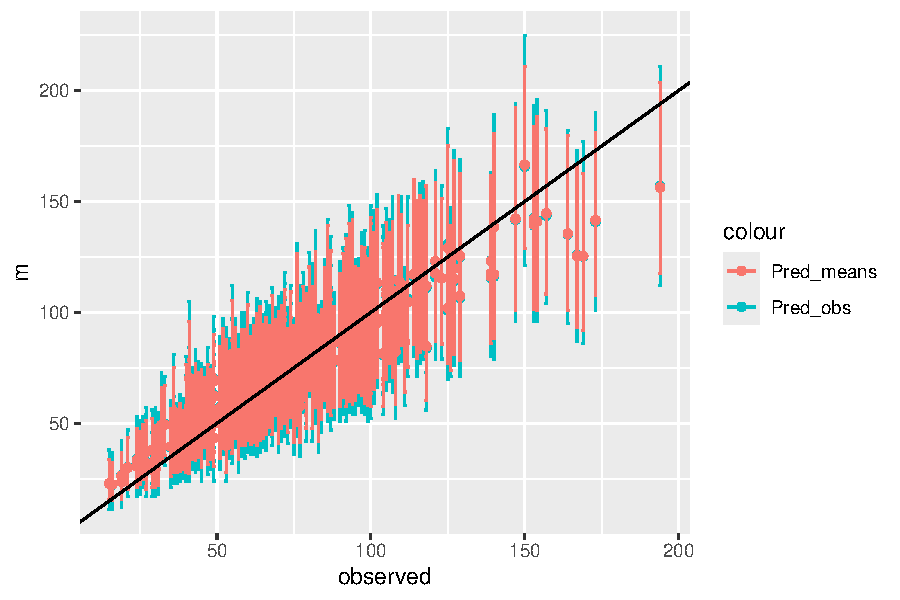
\includegraphics[keepaspectratio]{day3_practical_5_files/figure-pdf/unnamed-chunk-13-1.pdf}}
\end{center}

\end{tcolorbox}

\section{Geostatistics}\label{geostatistics}

In this practical we are going to fit a geostatistical model. We will:

\begin{itemize}
\item
  Learn how to fit a geostatistical model in \texttt{inlabru}
\item
  Learn how to build a mesh for the SPDE representation
\item
  Learn how to add spatial covariates to the model
\item
  Learn how to do predictions
\item
  Learn how to simulate from the fitted model
\end{itemize}

\begin{center}\rule{0.5\linewidth}{0.5pt}\end{center}

Libraries to load:

\begin{Shaded}
\begin{Highlighting}[]
\FunctionTok{library}\NormalTok{(dplyr)}
\FunctionTok{library}\NormalTok{(INLA)}
\FunctionTok{library}\NormalTok{(inlabru) }
\FunctionTok{library}\NormalTok{(sf)}
\FunctionTok{library}\NormalTok{(terra)}


\CommentTok{\# load some libraries to generate nice map plots}
\FunctionTok{library}\NormalTok{(scico)}
\FunctionTok{library}\NormalTok{(ggplot2)}
\FunctionTok{library}\NormalTok{(patchwork)}
\FunctionTok{library}\NormalTok{(mapview)}
\FunctionTok{library}\NormalTok{(tidyterra)}
\end{Highlighting}
\end{Shaded}

\subsection{The data}\label{the-data-1}

In this practical, we will explore data on the Pacific Cod (\emph{Gadus
macrocephalus}) from a trawl survey in Queen Charlotte Sound. The
\texttt{pcod} dataset is available from the \texttt{sdmTMB} package and
contains the presence/absence records of the Pacific Cod during each
surveys along with the biomass density of Pacific cod in the area swept
(kg/Km\(^2\)). The \texttt{qcs\_grid} data contain the depth values
stored as \(2\times 2\) km grid for Queen Charlotte Sound.

The dataset contains presence/absence data from 2003 to 2017. In this
practical we only consider year 2003.

We first load the dataset and select the year of interest

\begin{Shaded}
\begin{Highlighting}[]
\FunctionTok{library}\NormalTok{(sdmTMB)}

\NormalTok{pcod\_df }\OtherTok{=}\NormalTok{ sdmTMB}\SpecialCharTok{::}\NormalTok{pcod }\SpecialCharTok{\%\textgreater{}\%} \FunctionTok{filter}\NormalTok{(year}\SpecialCharTok{==}\DecValTok{2003}\NormalTok{)}
\NormalTok{qcs\_grid }\OtherTok{=}\NormalTok{ sdmTMB}\SpecialCharTok{::}\NormalTok{qcs\_grid}
\end{Highlighting}
\end{Shaded}

Then, we create ab \texttt{sf} object and assign the rough coordinate
reference to it:

\begin{Shaded}
\begin{Highlighting}[]
\NormalTok{pcod\_sf }\OtherTok{=}   \FunctionTok{st\_as\_sf}\NormalTok{(pcod\_df, }\AttributeTok{coords =} \FunctionTok{c}\NormalTok{(}\StringTok{"lon"}\NormalTok{,}\StringTok{"lat"}\NormalTok{), }\AttributeTok{crs =} \DecValTok{4326}\NormalTok{)}
\NormalTok{pcod\_sf }\OtherTok{=} \FunctionTok{st\_transform}\NormalTok{(pcod\_sf,}
\AttributeTok{crs =} \StringTok{"+proj=utm +zone=9 +datum=WGS84 +no\_defs +type=crs +units=km"}\NormalTok{ )}
\end{Highlighting}
\end{Shaded}

We convert the covariate into a raster and assign the same coordinate
reference:

\begin{Shaded}
\begin{Highlighting}[]
\NormalTok{depth\_r }\OtherTok{\textless{}{-}} \FunctionTok{rast}\NormalTok{(qcs\_grid, }\AttributeTok{type =} \StringTok{"xyz"}\NormalTok{)}
\FunctionTok{crs}\NormalTok{(depth\_r) }\OtherTok{\textless{}{-}} \FunctionTok{crs}\NormalTok{(pcod\_sf)}
\end{Highlighting}
\end{Shaded}

Finally we can plot our dataset. Note that to plot the raster we need to
upload also the \texttt{tidyterra} library.

\begin{Shaded}
\begin{Highlighting}[]
\FunctionTok{ggplot}\NormalTok{()}\SpecialCharTok{+} 
  \FunctionTok{geom\_spatraster}\NormalTok{(}\AttributeTok{data=}\NormalTok{depth\_r}\SpecialCharTok{$}\NormalTok{depth)}\SpecialCharTok{+}
  \FunctionTok{geom\_sf}\NormalTok{(}\AttributeTok{data=}\NormalTok{pcod\_sf,}\FunctionTok{aes}\NormalTok{(}\AttributeTok{color=}\FunctionTok{factor}\NormalTok{(present))) }\SpecialCharTok{+}
    \FunctionTok{scale\_color\_manual}\NormalTok{(}\AttributeTok{name=}\StringTok{"Occupancy status for the Pacific Cod"}\NormalTok{,}
                     \AttributeTok{values =} \FunctionTok{c}\NormalTok{(}\StringTok{"black"}\NormalTok{,}\StringTok{"orange"}\NormalTok{),}
                     \AttributeTok{labels=} \FunctionTok{c}\NormalTok{(}\StringTok{"Absence"}\NormalTok{,}\StringTok{"Presence"}\NormalTok{))}\SpecialCharTok{+}
  \FunctionTok{scale\_fill\_scico}\NormalTok{(}\AttributeTok{name =} \StringTok{"Depth"}\NormalTok{,}
                   \AttributeTok{palette =} \StringTok{"nuuk"}\NormalTok{,}
                   \AttributeTok{na.value =} \StringTok{"transparent"}\NormalTok{ ) }\SpecialCharTok{+} \FunctionTok{xlab}\NormalTok{(}\StringTok{""}\NormalTok{) }\SpecialCharTok{+} \FunctionTok{ylab}\NormalTok{(}\StringTok{""}\NormalTok{)}
\end{Highlighting}
\end{Shaded}

\pandocbounded{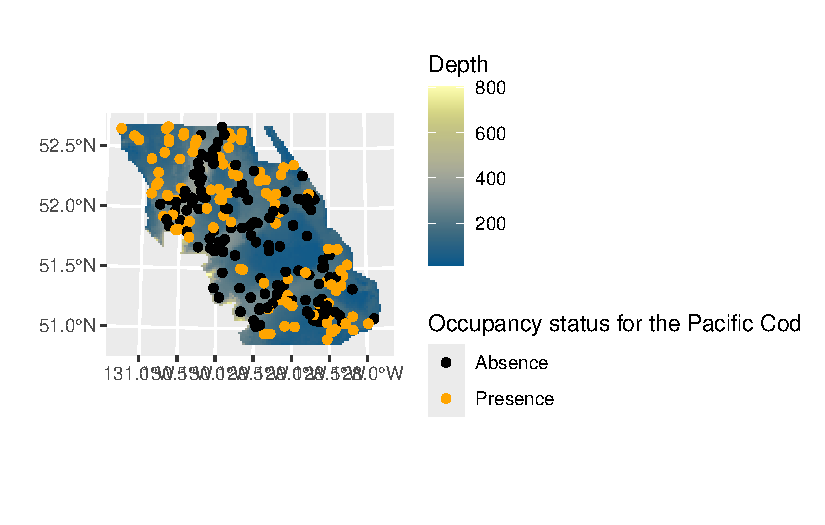
\includegraphics[keepaspectratio]{day3_practical_5_files/figure-pdf/unnamed-chunk-34-1.pdf}}

\subsection{The model}\label{the-model-1}

We first fit a simple model where we consider the observation as
Bernoulli and where the linear predictor contains only one intercept and
the GR field defined through the SPDE approach. The model is defined as:

\textbf{Stage 1} Model for the response

\[
y(s)|\eta(s)\sim\text{Binom}(1, p(s))
\] \textbf{Stage 2} Latent field model

\[
\eta(s) = \text{logit}(p(s)) = \beta_0 + \omega(s)
\]

with

\[
\omega(s)\sim \text{  GF with range } \rho\  \text{ and maginal variance }\ \sigma^2
\]

\textbf{Stage 3} Hyperparameters

The hyperparameters of the model are \(\rho\) and \(\sigma\)

\textbf{NOTE} In this case the linear predictor \(\eta\) consists of two
components!!

\subsubsection{The workflow}\label{the-workflow}

When fitting a geostatistical model we need to fulfill the following
tasks:

\begin{enumerate}
\def\labelenumi{\arabic{enumi}.}
\item
  Build the mesh
\item
  Define the SPDE representation of the spatial GF. This includes
  defining the priors for the range and sd of the spatial GF
\item
  Define the \emph{components} of the linear predictor. This includes
  the spatial GF and all eventual covariates
\item
  Define the observation model using the \texttt{bru\_obs()} function
\item
  Run the model using the \texttt{bru()} function
\end{enumerate}

\subsubsection{1. Building the mesh}\label{building-the-mesh}

The first task, when dealing with geostatistical models in
\texttt{inlabru} is to build the mesh that covers the area of interest.
For this purpose we use the function \texttt{fm\_messh\_2d}.

One way to build the mesh is to start from the locations where we have
observations, these are contained in the dataset \texttt{pcod\_sf}.

\begin{Shaded}
\begin{Highlighting}[]
\NormalTok{mesh }\OtherTok{=} \FunctionTok{fm\_mesh\_2d}\NormalTok{(}\AttributeTok{loc =}\NormalTok{ pcod\_sf,           }\CommentTok{\# Build the mesh}
                  \AttributeTok{max.edge =} \FunctionTok{c}\NormalTok{(}\DecValTok{10}\NormalTok{,}\DecValTok{20}\NormalTok{),     }\CommentTok{\# The largest allowed triangle edge length.}
                  \AttributeTok{offset =} \FunctionTok{c}\NormalTok{(}\DecValTok{5}\NormalTok{,}\DecValTok{50}\NormalTok{))       }\CommentTok{\# The automatic extension distance}
\FunctionTok{ggplot}\NormalTok{() }\SpecialCharTok{+} \FunctionTok{gg}\NormalTok{(mesh) }\SpecialCharTok{+} \FunctionTok{geom\_sf}\NormalTok{(}\AttributeTok{data=}\NormalTok{ pcod\_sf, }\FunctionTok{aes}\NormalTok{(}\AttributeTok{color =} \FunctionTok{factor}\NormalTok{(present)), }\AttributeTok{size =} \FloatTok{0.1}\NormalTok{) }\SpecialCharTok{+} \FunctionTok{xlab}\NormalTok{(}\StringTok{""}\NormalTok{) }\SpecialCharTok{+} \FunctionTok{ylab}\NormalTok{(}\StringTok{""}\NormalTok{)}
\end{Highlighting}
\end{Shaded}

\pandocbounded{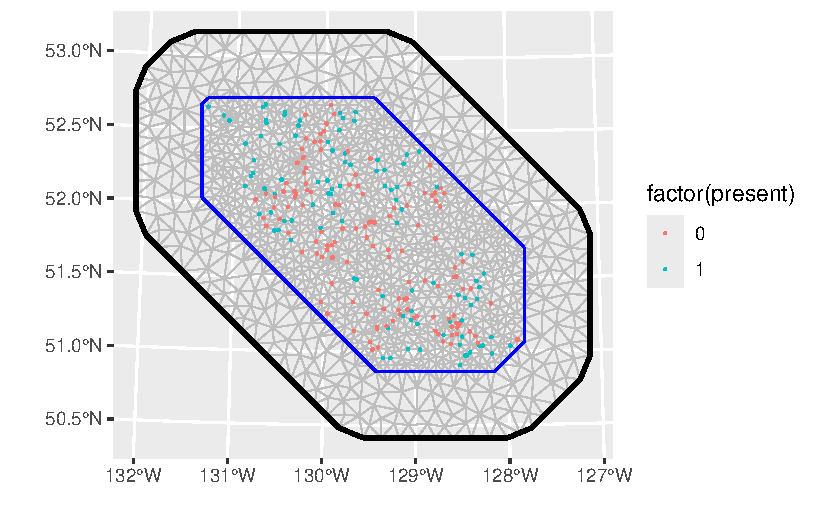
\includegraphics[keepaspectratio]{day3_practical_5_files/figure-pdf/unnamed-chunk-35-1.pdf}}

As you can see from the plot above, some of the locations are very close
to each other, this causes some very small triangles. This can be
avoided using the option \texttt{cutoff\ =} which collapses the
locations that are closer than a cutoff (those points are collapsed in
the mesh construction but, of course, not when it come to estimaation.)

\begin{Shaded}
\begin{Highlighting}[]
\NormalTok{mesh }\OtherTok{=} \FunctionTok{fm\_mesh\_2d}\NormalTok{(}\AttributeTok{loc =}\NormalTok{ pcod\_sf,           }\CommentTok{\# Build the mesh}
                  \AttributeTok{cutoff =} \DecValTok{2}\NormalTok{,}
                  \AttributeTok{max.edge =} \FunctionTok{c}\NormalTok{(}\DecValTok{10}\NormalTok{,}\DecValTok{20}\NormalTok{),     }\CommentTok{\# The largest allowed triangle edge length.}
                  \AttributeTok{offset =} \FunctionTok{c}\NormalTok{(}\DecValTok{5}\NormalTok{,}\DecValTok{50}\NormalTok{))       }\CommentTok{\# The automatic extension distance}
\FunctionTok{ggplot}\NormalTok{() }\SpecialCharTok{+} \FunctionTok{gg}\NormalTok{(mesh) }\SpecialCharTok{+} \FunctionTok{geom\_sf}\NormalTok{(}\AttributeTok{data=}\NormalTok{ pcod\_sf, }\FunctionTok{aes}\NormalTok{(}\AttributeTok{color =} \FunctionTok{factor}\NormalTok{(present)), }\AttributeTok{size =} \FloatTok{0.1}\NormalTok{) }\SpecialCharTok{+} \FunctionTok{xlab}\NormalTok{(}\StringTok{""}\NormalTok{) }\SpecialCharTok{+} \FunctionTok{ylab}\NormalTok{(}\StringTok{""}\NormalTok{)}
\end{Highlighting}
\end{Shaded}

\pandocbounded{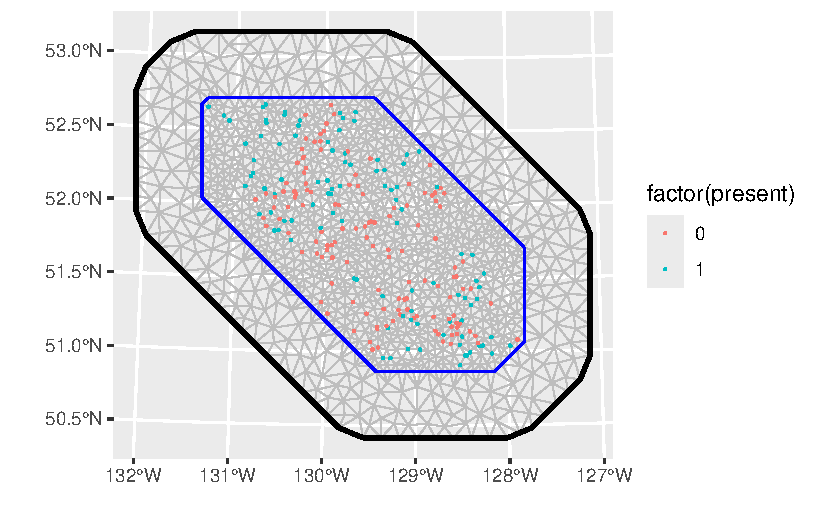
\includegraphics[keepaspectratio]{day3_practical_5_files/figure-pdf/unnamed-chunk-36-1.pdf}}

\begin{tcolorbox}[enhanced jigsaw, coltitle=black, bottomtitle=1mm, leftrule=.75mm, left=2mm, colback=white, colbacktitle=quarto-callout-warning-color!10!white, breakable, toptitle=1mm, titlerule=0mm, title={Task}, arc=.35mm, toprule=.15mm, bottomrule=.15mm, rightrule=.15mm, opacitybacktitle=0.6, opacityback=0, colframe=quarto-callout-warning-color-frame]

Look at the documentation for the \texttt{fm\_mesh\_2d} function typing

\begin{Shaded}
\begin{Highlighting}[]
\NormalTok{?fm\_mesh\_2d}
\end{Highlighting}
\end{Shaded}

play around with the different options and create different meshes.

The \emph{rule of thumb} is that your mesh should be:

\begin{itemize}
\tightlist
\item
  fine enough to well represent the spatial variability of your process,
  but not too fine in order to avoid computation burden
\item
  the triangles should be regular, avoid long and thin triangles.
\item
  The mesh should contain a buffer around your area of interest (this is
  what is defined in the \texttt{offset} option) in order to avoid
  boundary artefact in the estimated variance.
\end{itemize}

\end{tcolorbox}

\subsubsection{2. Define the SPDE representation of the spatial
GF}\label{define-the-spde-representation-of-the-spatial-gf}

To define the SPDE representation of the spatial GF we use the function
\texttt{inla.spde2.pcmatern}. This takes as input the mesh we have
defined and the PC-priors definition for \(\rho\) and \(\sigma\) (the
range and the marginal standard deviation of the field).

PC priors Gaussian Random field are defined in (Fuglstad et al.~2018).
From a practical perspective for the range \(\rho\) you need to define
two paramters \(\rho_0\) and \(p_{\rho}\) such that you believe it is
reasonable that

\[
P(\rho<\rho_0)=p_{\rho}
\]

while for the margianal variance \(\sigma\) you need to define two
parameters \(\sigma_0\) and \(p_{\sigma}\) such that you believe it is
reasonable that

\[
P(\sigma<\sigma_0)=p_{\sigma}
\]

You can use the following function to compute and plot the prior
distributions for the range and sd of the Matern field.

\begin{Shaded}
\begin{Highlighting}[]
\NormalTok{dens\_prior\_range }\OtherTok{=} \ControlFlowTok{function}\NormalTok{(rho\_0, p\_alpha)}
\NormalTok{\{}
  \CommentTok{\# compute the density of the PC prior for the}
  \CommentTok{\# range rho of the Matern field}
  \CommentTok{\# rho\_0 and p\_alpha are defined such that}
  \CommentTok{\# P(rho\textless{}rho\_0) = p\_alpha}
\NormalTok{  rho }\OtherTok{=} \FunctionTok{seq}\NormalTok{(}\DecValTok{0}\NormalTok{, rho\_0}\SpecialCharTok{*}\DecValTok{10}\NormalTok{, }\AttributeTok{length.out =}\DecValTok{100}\NormalTok{)}
\NormalTok{  alpha1\_tilde }\OtherTok{=} \SpecialCharTok{{-}}\FunctionTok{log}\NormalTok{(p\_alpha) }\SpecialCharTok{*}\NormalTok{ rho\_0}
\NormalTok{  dens\_rho }\OtherTok{=}\NormalTok{  alpha1\_tilde }\SpecialCharTok{/}\NormalTok{ rho}\SpecialCharTok{\^{}}\DecValTok{2} \SpecialCharTok{*} \FunctionTok{exp}\NormalTok{(}\SpecialCharTok{{-}}\NormalTok{alpha1\_tilde }\SpecialCharTok{/}\NormalTok{ rho)}
  \FunctionTok{return}\NormalTok{(}\FunctionTok{data.frame}\NormalTok{(}\AttributeTok{x =}\NormalTok{ rho, }\AttributeTok{y =}\NormalTok{ dens\_rho))}
\NormalTok{\}}

\NormalTok{dens\_prior\_sd }\OtherTok{=} \ControlFlowTok{function}\NormalTok{(sigma\_0, p\_sigma)}
\NormalTok{\{}
  \CommentTok{\# compute the density of the PC prior for the}
  \CommentTok{\# sd sigma of the Matern field}
  \CommentTok{\# sigma\_0 and p\_sigma are defined such that}
  \CommentTok{\# P(sigma\textgreater{}sigma\_0) = p\_sigma}
\NormalTok{  sigma }\OtherTok{=} \FunctionTok{seq}\NormalTok{(}\DecValTok{0}\NormalTok{, sigma\_0}\SpecialCharTok{*}\DecValTok{10}\NormalTok{, }\AttributeTok{length.out =}\DecValTok{100}\NormalTok{)}
\NormalTok{  alpha2\_tilde }\OtherTok{=} \SpecialCharTok{{-}}\FunctionTok{log}\NormalTok{(p\_sigma)}\SpecialCharTok{/}\NormalTok{sigma\_0}
\NormalTok{  dens\_sigma }\OtherTok{=}\NormalTok{ alpha2\_tilde}\SpecialCharTok{*} \FunctionTok{exp}\NormalTok{(}\SpecialCharTok{{-}}\NormalTok{alpha2\_tilde }\SpecialCharTok{*}\NormalTok{ sigma) }
  \FunctionTok{return}\NormalTok{(}\FunctionTok{data.frame}\NormalTok{(}\AttributeTok{x =}\NormalTok{ sigma, }\AttributeTok{y =}\NormalTok{ dens\_sigma))}
\NormalTok{\}}
\end{Highlighting}
\end{Shaded}

Here are some alternatives for defining priors for our model

\begin{Shaded}
\begin{Highlighting}[]
\NormalTok{spde\_model1 }\OtherTok{=}  \FunctionTok{inla.spde2.pcmatern}\NormalTok{(mesh,}
                                  \AttributeTok{prior.sigma =} \FunctionTok{c}\NormalTok{(.}\DecValTok{1}\NormalTok{, }\FloatTok{0.5}\NormalTok{),}
                                  \AttributeTok{prior.range =} \FunctionTok{c}\NormalTok{(}\DecValTok{30}\NormalTok{, }\FloatTok{0.5}\NormalTok{))}
\NormalTok{spde\_model2 }\OtherTok{=}  \FunctionTok{inla.spde2.pcmatern}\NormalTok{(mesh,}
                                  \AttributeTok{prior.sigma =} \FunctionTok{c}\NormalTok{(}\DecValTok{10}\NormalTok{, }\FloatTok{0.5}\NormalTok{),}
                                  \AttributeTok{prior.range =} \FunctionTok{c}\NormalTok{(}\DecValTok{1000}\NormalTok{, }\FloatTok{0.5}\NormalTok{))}
\NormalTok{spde\_model3 }\OtherTok{=}  \FunctionTok{inla.spde2.pcmatern}\NormalTok{(mesh,}
                                  \AttributeTok{prior.sigma =} \FunctionTok{c}\NormalTok{(}\DecValTok{1}\NormalTok{, }\FloatTok{0.5}\NormalTok{),}
                                  \AttributeTok{prior.range =} \FunctionTok{c}\NormalTok{(}\DecValTok{100}\NormalTok{, }\FloatTok{0.5}\NormalTok{))}
\end{Highlighting}
\end{Shaded}

And here we plot the different priors for the range:

\begin{Shaded}
\begin{Highlighting}[]
\FunctionTok{ggplot}\NormalTok{() }\SpecialCharTok{+} 
  \FunctionTok{geom\_line}\NormalTok{(}\AttributeTok{data =} \FunctionTok{dens\_prior\_range}\NormalTok{(}\DecValTok{30}\NormalTok{,.}\DecValTok{5}\NormalTok{), }\FunctionTok{aes}\NormalTok{(x,y, }\AttributeTok{color =} \StringTok{"model1"}\NormalTok{)) }\SpecialCharTok{+}
  \FunctionTok{geom\_line}\NormalTok{(}\AttributeTok{data =} \FunctionTok{dens\_prior\_range}\NormalTok{(}\DecValTok{1000}\NormalTok{,.}\DecValTok{5}\NormalTok{), }\FunctionTok{aes}\NormalTok{(x,y, }\AttributeTok{color =} \StringTok{"model2"}\NormalTok{)) }\SpecialCharTok{+}
  \FunctionTok{geom\_line}\NormalTok{(}\AttributeTok{data =} \FunctionTok{dens\_prior\_range}\NormalTok{(}\DecValTok{100}\NormalTok{,.}\DecValTok{5}\NormalTok{), }\FunctionTok{aes}\NormalTok{(x,y, }\AttributeTok{color =} \StringTok{"model3"}\NormalTok{)) }
\end{Highlighting}
\end{Shaded}

\pandocbounded{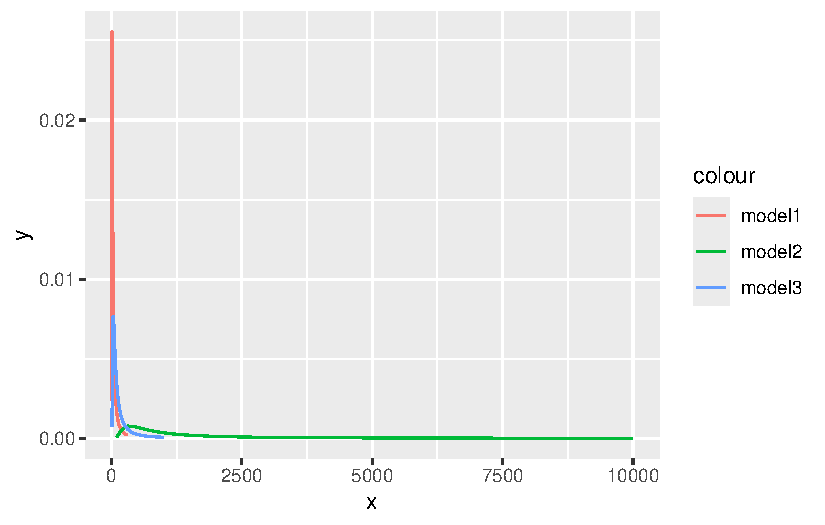
\includegraphics[keepaspectratio]{day3_practical_5_files/figure-pdf/unnamed-chunk-40-1.pdf}}

and for the sd:

\begin{Shaded}
\begin{Highlighting}[]
\FunctionTok{ggplot}\NormalTok{() }\SpecialCharTok{+} 
  \FunctionTok{geom\_line}\NormalTok{(}\AttributeTok{data =} \FunctionTok{dens\_prior\_sd}\NormalTok{(}\DecValTok{1}\NormalTok{,.}\DecValTok{5}\NormalTok{), }\FunctionTok{aes}\NormalTok{(x,y, }\AttributeTok{color =} \StringTok{"model1"}\NormalTok{)) }\SpecialCharTok{+}
  \FunctionTok{geom\_line}\NormalTok{(}\AttributeTok{data =} \FunctionTok{dens\_prior\_sd}\NormalTok{(}\DecValTok{10}\NormalTok{,.}\DecValTok{5}\NormalTok{), }\FunctionTok{aes}\NormalTok{(x,y, }\AttributeTok{color =} \StringTok{"model2"}\NormalTok{)) }\SpecialCharTok{+}
  \FunctionTok{geom\_line}\NormalTok{(}\AttributeTok{data =} \FunctionTok{dens\_prior\_sd}\NormalTok{(.}\DecValTok{1}\NormalTok{,.}\DecValTok{5}\NormalTok{), }\FunctionTok{aes}\NormalTok{(x,y, }\AttributeTok{color =} \StringTok{"model3"}\NormalTok{)) }
\end{Highlighting}
\end{Shaded}

\pandocbounded{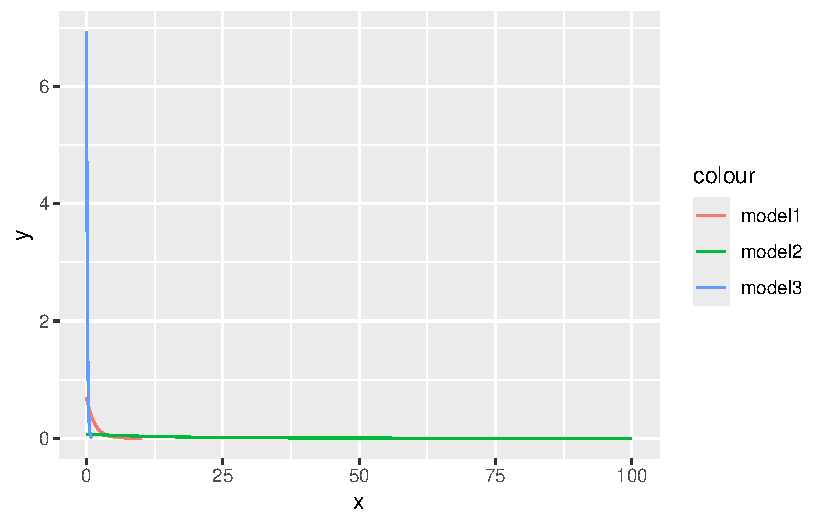
\includegraphics[keepaspectratio]{day3_practical_5_files/figure-pdf/unnamed-chunk-41-1.pdf}}

\begin{tcolorbox}[enhanced jigsaw, coltitle=black, bottomtitle=1mm, leftrule=.75mm, left=2mm, colback=white, colbacktitle=quarto-callout-tip-color!10!white, breakable, toptitle=1mm, titlerule=0mm, title={Question}, arc=.35mm, toprule=.15mm, bottomrule=.15mm, rightrule=.15mm, opacitybacktitle=0.6, opacityback=0, colframe=quarto-callout-tip-color-frame]

Consider the \texttt{pcod\_sf}, the spatial extension and type of the
data\ldots is some of the previous choices more reasonable than other?

\begin{itemize}
\tightlist
\item
  \begin{enumerate}
  \def\labelenumi{(\Alph{enumi})}
  \tightlist
  \item
    spde\_model1\\
  \end{enumerate}
\item
  \begin{enumerate}
  \def\labelenumi{(\Alph{enumi})}
  \setcounter{enumi}{1}
  \tightlist
  \item
    spde\_model2\\
  \end{enumerate}
\item
  \begin{enumerate}
  \def\labelenumi{(\Alph{enumi})}
  \setcounter{enumi}{2}
  \tightlist
  \item
    spde\_model3
  \end{enumerate}
\end{itemize}

\textbf{NOTE} Remember that a prior should be reasonable..but the model
should not totally depend on it.

\end{tcolorbox}

\subsubsection{3. Define the components of the linear
predictor}\label{define-the-components-of-the-linear-predictor}

We have now defined a mesh and a SPDE representation of the spatial GF.
We now need to define the model components:

\begin{Shaded}
\begin{Highlighting}[]
\NormalTok{cmp }\OtherTok{=} \ErrorTok{\textasciitilde{}} \FunctionTok{Intercept}\NormalTok{(}\DecValTok{1}\NormalTok{) }\SpecialCharTok{+} \FunctionTok{space}\NormalTok{(geometry, }\AttributeTok{model =}\NormalTok{ spde\_model3)}
\end{Highlighting}
\end{Shaded}

\textbf{NOTE} since the dataframe we use (\texttt{pcod\_sf}) is an
\texttt{sf} object the input in the \texttt{space()} component is the
geometry of the dataset.

\subsubsection{4. Define the observation
model}\label{define-the-observation-model}

Our data are Bernoulli distributed so we can define the observation
model as:

\begin{Shaded}
\begin{Highlighting}[]
\NormalTok{formula }\OtherTok{=}\NormalTok{ present }\SpecialCharTok{\textasciitilde{}}\NormalTok{ Intercept  }\SpecialCharTok{+}\NormalTok{ space}

\NormalTok{lik }\OtherTok{=} \FunctionTok{bru\_obs}\NormalTok{(}\AttributeTok{formula =}\NormalTok{ formula, }
              \AttributeTok{data =}\NormalTok{ pcod\_sf, }
              \AttributeTok{family =} \StringTok{"binomial"}\NormalTok{)}
\end{Highlighting}
\end{Shaded}

\subsubsection{5. Run the model}\label{run-the-model}

Finally we are ready to run the model

\begin{Shaded}
\begin{Highlighting}[]
\NormalTok{fit1 }\OtherTok{=} \FunctionTok{bru}\NormalTok{(cmp,lik)}
\end{Highlighting}
\end{Shaded}

\subsection{Extract results}\label{extract-results}

\subsubsection{Hyperparameters}\label{hyperparameters}

\begin{tcolorbox}[enhanced jigsaw, coltitle=black, bottomtitle=1mm, leftrule=.75mm, left=2mm, colback=white, colbacktitle=quarto-callout-warning-color!10!white, breakable, toptitle=1mm, titlerule=0mm, title={Task}, arc=.35mm, toprule=.15mm, bottomrule=.15mm, rightrule=.15mm, opacitybacktitle=0.6, opacityback=0, colframe=quarto-callout-warning-color-frame]

Plot the posterior densities for the range \(\rho\) and the standard
deviation \(\sigma\) alog with the prior for both parameters.

Take hint

Posterior marginals for the hyperparameters can be extracted from the
fitted model as:

Click here to see the solution

\begin{Shaded}
\begin{Highlighting}[]
\NormalTok{fit1}\SpecialCharTok{$}\NormalTok{marginals.hyperpar}\SpecialCharTok{$}\StringTok{\textquotesingle{}name of the parameter\textquotesingle{}}
\end{Highlighting}
\end{Shaded}

Click here to see the solution

\begin{Shaded}
\begin{Highlighting}[]
\CommentTok{\# Extract marginal for the range}

\FunctionTok{ggplot}\NormalTok{() }\SpecialCharTok{+} 
  \FunctionTok{geom\_line}\NormalTok{(}\AttributeTok{data =}\NormalTok{ fit1}\SpecialCharTok{$}\NormalTok{marginals.hyperpar}\SpecialCharTok{$}\StringTok{\textasciigrave{}}\AttributeTok{Range for space}\StringTok{\textasciigrave{}}\NormalTok{,}
            \FunctionTok{aes}\NormalTok{(x,y, }\AttributeTok{color =} \StringTok{"Posterior"}\NormalTok{)) }\SpecialCharTok{+}
  \FunctionTok{geom\_line}\NormalTok{(}\AttributeTok{data =} \FunctionTok{dens\_prior\_range}\NormalTok{(}\DecValTok{100}\NormalTok{,.}\DecValTok{5}\NormalTok{),}
            \FunctionTok{aes}\NormalTok{(x,y, }\AttributeTok{color =} \StringTok{"Prior"}\NormalTok{))}


\FunctionTok{ggplot}\NormalTok{() }\SpecialCharTok{+} 
  \FunctionTok{geom\_line}\NormalTok{(}\AttributeTok{data =}\NormalTok{ fit1}\SpecialCharTok{$}\NormalTok{marginals.hyperpar}\SpecialCharTok{$}\StringTok{\textasciigrave{}}\AttributeTok{Stdev for space}\StringTok{\textasciigrave{}}\NormalTok{,}
            \FunctionTok{aes}\NormalTok{(x,y, }\AttributeTok{color =} \StringTok{"Posterior"}\NormalTok{)) }\SpecialCharTok{+}
  \FunctionTok{geom\_line}\NormalTok{(}\AttributeTok{data =} \FunctionTok{dens\_prior\_sd}\NormalTok{(}\DecValTok{1}\NormalTok{,.}\DecValTok{5}\NormalTok{), }\FunctionTok{aes}\NormalTok{(x,y, }\AttributeTok{color =} \StringTok{"Prior"}\NormalTok{))}
\end{Highlighting}
\end{Shaded}

\end{tcolorbox}

\subsection{Spatial prediction}\label{spatial-prediction}

We now want to extract the estimated posterior mean and sd of spatial
GF. To do this we first need to define a grid of points where we want to
predict. We do this using the function \texttt{fm\_pixel()} which
creates a regular grid of points covering the mesh

\begin{Shaded}
\begin{Highlighting}[]
\NormalTok{pxl }\OtherTok{=} \FunctionTok{fm\_pixels}\NormalTok{(mesh)}
\end{Highlighting}
\end{Shaded}

then compute the prediction for both the spatial GF and the linear
predictor (spatial GF + intercept)

\begin{Shaded}
\begin{Highlighting}[]
\NormalTok{preds }\OtherTok{=} \FunctionTok{predict}\NormalTok{(fit1, pxl, }\SpecialCharTok{\textasciitilde{}}\FunctionTok{data.frame}\NormalTok{(}\AttributeTok{spatial =}\NormalTok{ space,}
                                      \AttributeTok{total =}\NormalTok{ Intercept }\SpecialCharTok{+}\NormalTok{ space))}
\end{Highlighting}
\end{Shaded}

Finally, we can plot the maps

\begin{Shaded}
\begin{Highlighting}[]
\FunctionTok{ggplot}\NormalTok{() }\SpecialCharTok{+} \FunctionTok{geom\_sf}\NormalTok{(}\AttributeTok{data =}\NormalTok{ preds}\SpecialCharTok{$}\NormalTok{spatial,}\FunctionTok{aes}\NormalTok{(}\AttributeTok{color =}\NormalTok{ mean)) }\SpecialCharTok{+} \FunctionTok{scale\_color\_scico}\NormalTok{() }\SpecialCharTok{+} \FunctionTok{ggtitle}\NormalTok{(}\StringTok{"Posterior mean"}\NormalTok{)}
\end{Highlighting}
\end{Shaded}

\pandocbounded{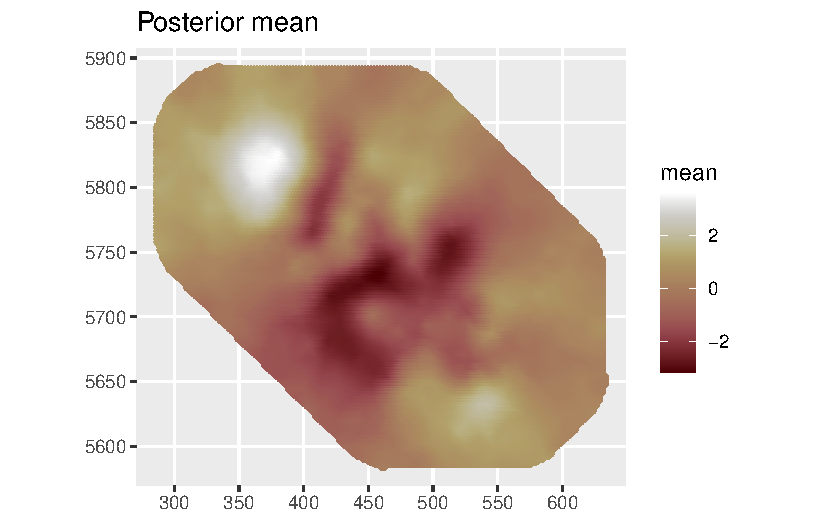
\includegraphics[keepaspectratio]{day3_practical_5_files/figure-pdf/unnamed-chunk-49-1.pdf}}

\begin{Shaded}
\begin{Highlighting}[]
\FunctionTok{ggplot}\NormalTok{() }\SpecialCharTok{+} \FunctionTok{geom\_sf}\NormalTok{(}\AttributeTok{data =}\NormalTok{ preds}\SpecialCharTok{$}\NormalTok{spatial,}\FunctionTok{aes}\NormalTok{(}\AttributeTok{color =}\NormalTok{ sd)) }\SpecialCharTok{+} \FunctionTok{scale\_color\_scico}\NormalTok{() }\SpecialCharTok{+} \FunctionTok{ggtitle}\NormalTok{(}\StringTok{"Posterior sd"}\NormalTok{)}
\end{Highlighting}
\end{Shaded}

\pandocbounded{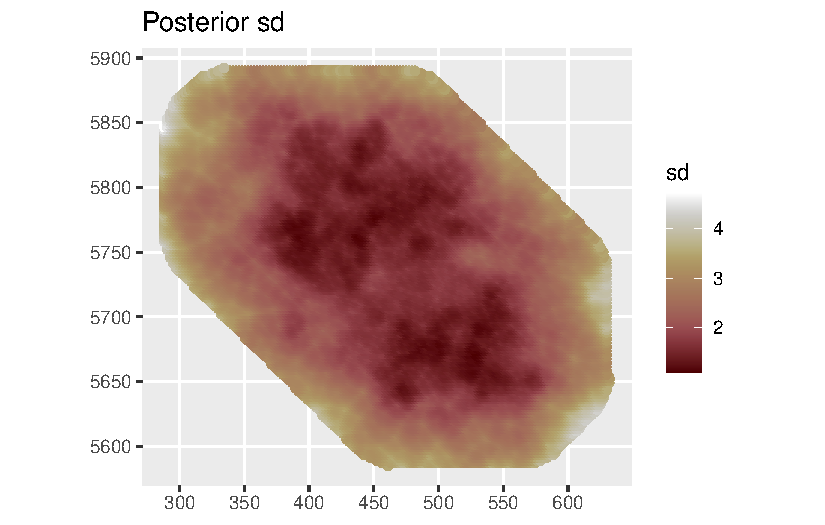
\includegraphics[keepaspectratio]{day3_practical_5_files/figure-pdf/unnamed-chunk-49-2.pdf}}

\textbf{Note} The posterior sd is lowest at the observation points. Note
how the posterior sd is inflated around the border, this is the ``border
effect'' due to the SPDE representation.

Instead of predicting over a grid covering the whole mesh, we can limit
our predictions to the points where the covariate is defined. We can do
this by defining a \texttt{sf} object using coordinates in the object
\texttt{depth\_r}.

\begin{Shaded}
\begin{Highlighting}[]
\NormalTok{pxl1 }\OtherTok{=} \FunctionTok{data.frame}\NormalTok{(}\FunctionTok{crds}\NormalTok{(depth\_r), }
                  \FunctionTok{as.data.frame}\NormalTok{(depth\_r}\SpecialCharTok{$}\NormalTok{depth)) }\SpecialCharTok{\%\textgreater{}\%} 
       \FunctionTok{filter}\NormalTok{(}\SpecialCharTok{!}\FunctionTok{is.na}\NormalTok{(depth)) }\SpecialCharTok{\%\textgreater{}\%}
\FunctionTok{st\_as\_sf}\NormalTok{(}\AttributeTok{coords =} \FunctionTok{c}\NormalTok{(}\StringTok{"x"}\NormalTok{,}\StringTok{"y"}\NormalTok{))}
\end{Highlighting}
\end{Shaded}

\begin{tcolorbox}[enhanced jigsaw, coltitle=black, bottomtitle=1mm, leftrule=.75mm, left=2mm, colback=white, colbacktitle=quarto-callout-warning-color!10!white, breakable, toptitle=1mm, titlerule=0mm, title={Task}, arc=.35mm, toprule=.15mm, bottomrule=.15mm, rightrule=.15mm, opacitybacktitle=0.6, opacityback=0, colframe=quarto-callout-warning-color-frame]

Produce prediction over \texttt{pxl1} unsing the same techniques as
before. Plot your results.

Take hint

Add hint details here\ldots{}

Click here to see the solution

\begin{Shaded}
\begin{Highlighting}[]
\NormalTok{pred\_pxl1 }\OtherTok{=} \FunctionTok{predict}\NormalTok{(fit1, pxl1, }\SpecialCharTok{\textasciitilde{}}\FunctionTok{data.frame}\NormalTok{(}\AttributeTok{spatial =}\NormalTok{ space,}
                                      \AttributeTok{total =}\NormalTok{ Intercept }\SpecialCharTok{+}\NormalTok{ space))}

\FunctionTok{ggplot}\NormalTok{() }\SpecialCharTok{+} \FunctionTok{geom\_sf}\NormalTok{(}\AttributeTok{data =}\NormalTok{ pred\_pxl1}\SpecialCharTok{$}\NormalTok{total,}\FunctionTok{aes}\NormalTok{(}\AttributeTok{color =}\NormalTok{ mean)) }\SpecialCharTok{+} \FunctionTok{scale\_color\_scico}\NormalTok{() }\SpecialCharTok{+} \FunctionTok{ggtitle}\NormalTok{(}\StringTok{"Posterior mean"}\NormalTok{)}
\end{Highlighting}
\end{Shaded}

\begin{center}
\pandocbounded{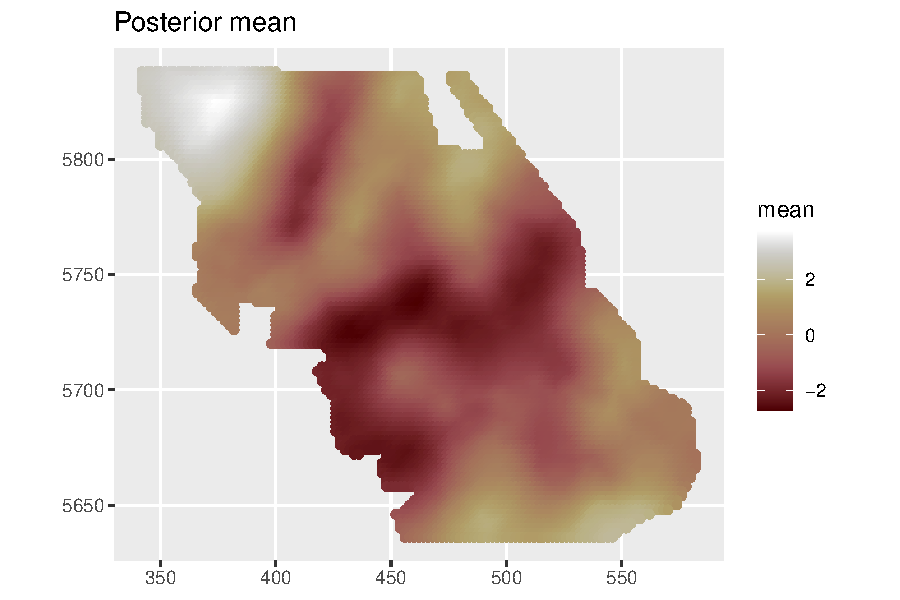
\includegraphics[keepaspectratio]{day3_practical_5_files/figure-pdf/unnamed-chunk-51-1.pdf}}
\end{center}

\begin{Shaded}
\begin{Highlighting}[]
\FunctionTok{ggplot}\NormalTok{() }\SpecialCharTok{+} \FunctionTok{geom\_sf}\NormalTok{(}\AttributeTok{data =}\NormalTok{ pred\_pxl1}\SpecialCharTok{$}\NormalTok{total,}\FunctionTok{aes}\NormalTok{(}\AttributeTok{color =}\NormalTok{ sd)) }\SpecialCharTok{+} \FunctionTok{scale\_color\_scico}\NormalTok{() }\SpecialCharTok{+} \FunctionTok{ggtitle}\NormalTok{(}\StringTok{"Posterior sd"}\NormalTok{)}
\end{Highlighting}
\end{Shaded}

\begin{center}
\pandocbounded{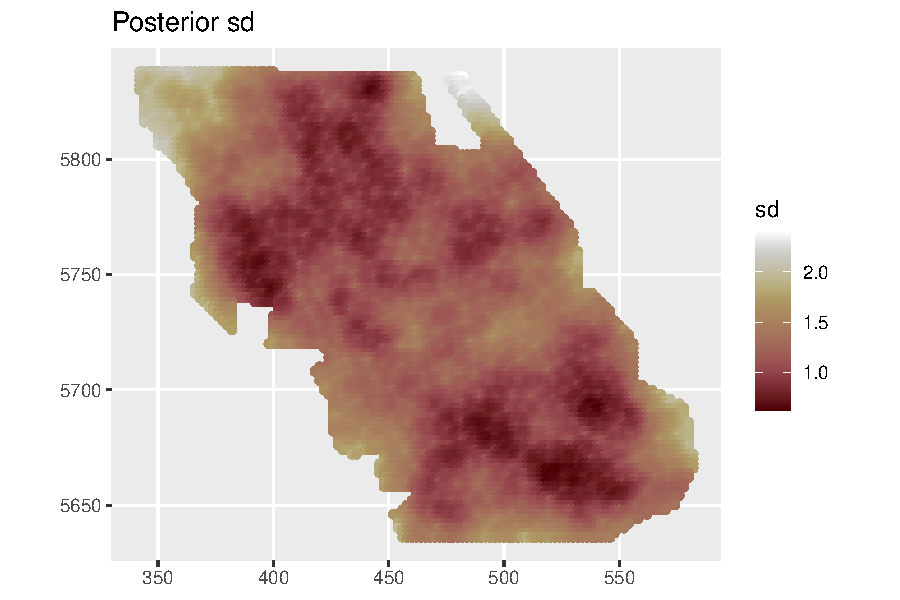
\includegraphics[keepaspectratio]{day3_practical_5_files/figure-pdf/unnamed-chunk-51-2.pdf}}
\end{center}

\end{tcolorbox}

Instead of computing the posterior mean and standard deviations of the
estimated surface, one can also \emph{simulate} possible realizations of
such surface. This will give the user a better idea of the type of
realized surfaces one can expect. We can do this using the function
\texttt{generate()}.

\begin{Shaded}
\begin{Highlighting}[]
\CommentTok{\# we simulate 4 samples from the }
\NormalTok{gens }\OtherTok{=} \FunctionTok{generate}\NormalTok{(fit1, pxl1, }\SpecialCharTok{\textasciitilde{}}\NormalTok{ (Intercept }\SpecialCharTok{+}\NormalTok{ space),}
                \AttributeTok{n.samples =} \DecValTok{4}\NormalTok{)}

\NormalTok{pp }\OtherTok{=} \FunctionTok{cbind}\NormalTok{(pxl1, gens)}

\NormalTok{pp }\SpecialCharTok{\%\textgreater{}\%} \FunctionTok{select}\NormalTok{(}\SpecialCharTok{{-}}\NormalTok{depth) }\SpecialCharTok{\%\textgreater{}\%}
  \FunctionTok{pivot\_longer}\NormalTok{(}\SpecialCharTok{{-}}\NormalTok{geometry) }\SpecialCharTok{\%\textgreater{}\%}
    \FunctionTok{ggplot}\NormalTok{() }\SpecialCharTok{+} 
      \FunctionTok{geom\_sf}\NormalTok{(}\FunctionTok{aes}\NormalTok{(}\AttributeTok{color =}\NormalTok{ value)) }\SpecialCharTok{+}
      \FunctionTok{facet\_wrap}\NormalTok{(.}\SpecialCharTok{\textasciitilde{}}\NormalTok{name) }\SpecialCharTok{+}
        \FunctionTok{scale\_color\_scico}\NormalTok{(}\AttributeTok{direction =} \SpecialCharTok{{-}}\DecValTok{1}\NormalTok{) }\SpecialCharTok{+}
        \FunctionTok{ggtitle}\NormalTok{(}\StringTok{"Sample from the fitted model"}\NormalTok{)}
\end{Highlighting}
\end{Shaded}

\pandocbounded{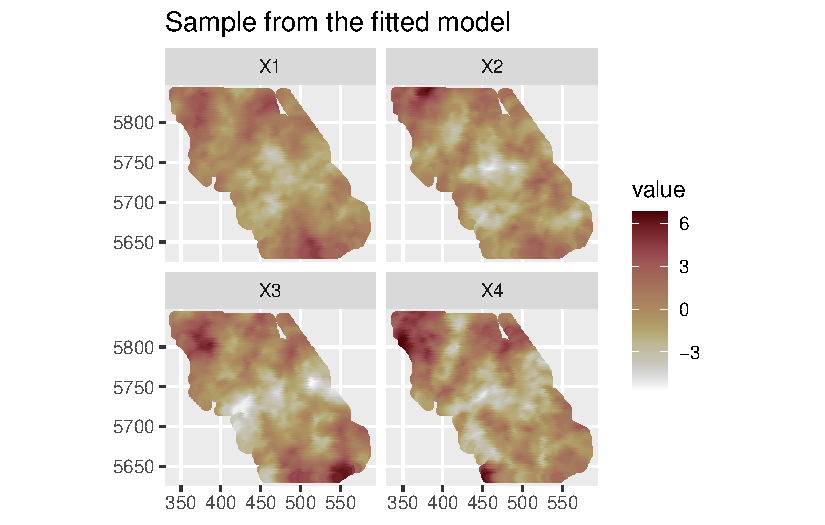
\includegraphics[keepaspectratio]{day3_practical_5_files/figure-pdf/unnamed-chunk-52-1.pdf}}

\subsection{An alternative model}\label{an-alternative-model}

We now want to check if the \texttt{depth} covatiate has an influende on
the probability of presence. We do this in two different models

\begin{enumerate}
\def\labelenumi{\arabic{enumi}.}
\tightlist
\item
  \textbf{Model 1} The depth enters the model in a linear way. The
  linear predictor is then defined as:
\end{enumerate}

\[
  \eta(s) = \text{logit}(p(s)) = \beta_0 + \omega(s) + \beta_1\ \text{depth}(s)
\]

\begin{enumerate}
\def\labelenumi{\arabic{enumi}.}
\setcounter{enumi}{1}
\tightlist
\item
  \textbf{Model 1} The depth enters the model in a non linear way. The
  linear predictor is then defined as:
\end{enumerate}

\[
  \eta(s) = \text{logit}(p(s)) = \beta_0 + \omega(s) +  f(\text{depth}(s))
\] where \(f(.)\) is a smooth function. We will use a RW2 model for
this.

\begin{tcolorbox}[enhanced jigsaw, coltitle=black, bottomtitle=1mm, leftrule=.75mm, left=2mm, colback=white, colbacktitle=quarto-callout-warning-color!10!white, breakable, toptitle=1mm, titlerule=0mm, title={Task}, arc=.35mm, toprule=.15mm, bottomrule=.15mm, rightrule=.15mm, opacitybacktitle=0.6, opacityback=0, colframe=quarto-callout-warning-color-frame]

Fit model 1. Define components, observation model and use the
\texttt{bru()} function to estimate the parameters.

\textbf{Note} Use the scaled version of the covariate stored in
\texttt{depth\_r\$depth\_scaled}.

What is the liner effect of depth on the logit probability?

Take hint

Add hint details here\ldots{}

Click here to see the solution

\begin{Shaded}
\begin{Highlighting}[]
\NormalTok{cmp }\OtherTok{=} \ErrorTok{\textasciitilde{}} \FunctionTok{Intercept}\NormalTok{(}\DecValTok{1}\NormalTok{) }\SpecialCharTok{+} \FunctionTok{space}\NormalTok{(geometry, }\AttributeTok{model =}\NormalTok{ spde\_model3) }\SpecialCharTok{+}
        \FunctionTok{covariate}\NormalTok{(depth\_r}\SpecialCharTok{$}\NormalTok{depth\_scaled, }\AttributeTok{model =} \StringTok{"linear"}\NormalTok{)}

\NormalTok{formula }\OtherTok{=}\NormalTok{ present }\SpecialCharTok{\textasciitilde{}}\NormalTok{ Intercept  }\SpecialCharTok{+}\NormalTok{ space }\SpecialCharTok{+}\NormalTok{ covariate}

\NormalTok{lik }\OtherTok{=} \FunctionTok{bru\_obs}\NormalTok{(}\AttributeTok{formula =}\NormalTok{ formula, }
              \AttributeTok{data =}\NormalTok{ pcod\_sf, }
              \AttributeTok{family =} \StringTok{"binomial"}\NormalTok{)}


\NormalTok{fit2 }\OtherTok{=} \FunctionTok{bru}\NormalTok{(cmp, lik)}
\end{Highlighting}
\end{Shaded}

\end{tcolorbox}

We now want to fit \textbf{Model 2} where we allow the effect of depth
to be non-linear. To use the RW2 model we need to \emph{group} the
values of depth into distinct classe. To do this we use the function
\texttt{inla.group()} which, by default, creates 20 groups. The we can
fit the model as usual

\begin{Shaded}
\begin{Highlighting}[]
\CommentTok{\# create the grouped variable}
\NormalTok{depth\_r}\SpecialCharTok{$}\NormalTok{depth\_group }\OtherTok{=} \FunctionTok{inla.group}\NormalTok{(}\FunctionTok{values}\NormalTok{(depth\_r}\SpecialCharTok{$}\NormalTok{depth\_scaled))}

\CommentTok{\# run the model}
\NormalTok{cmp }\OtherTok{=} \ErrorTok{\textasciitilde{}} \FunctionTok{Intercept}\NormalTok{(}\DecValTok{1}\NormalTok{) }\SpecialCharTok{+} \FunctionTok{space}\NormalTok{(geometry, }\AttributeTok{model =}\NormalTok{ spde\_model3) }\SpecialCharTok{+}
        \FunctionTok{covariate}\NormalTok{(depth\_r}\SpecialCharTok{$}\NormalTok{depth\_group, }\AttributeTok{model =} \StringTok{"rw2"}\NormalTok{)}

\NormalTok{formula }\OtherTok{=}\NormalTok{ present }\SpecialCharTok{\textasciitilde{}}\NormalTok{ Intercept  }\SpecialCharTok{+}\NormalTok{ space }\SpecialCharTok{+}\NormalTok{ covariate}

\NormalTok{lik }\OtherTok{=} \FunctionTok{bru\_obs}\NormalTok{(}\AttributeTok{formula =}\NormalTok{ formula, }
              \AttributeTok{data =}\NormalTok{ pcod\_sf, }
              \AttributeTok{family =} \StringTok{"binomial"}\NormalTok{)}


\NormalTok{fit3 }\OtherTok{=} \FunctionTok{bru}\NormalTok{(cmp, lik)}

\CommentTok{\# plot the estimated effect of depth}

\NormalTok{fit3}\SpecialCharTok{$}\NormalTok{summary.random}\SpecialCharTok{$}\NormalTok{covariate }\SpecialCharTok{\%\textgreater{}\%} 
  \FunctionTok{ggplot}\NormalTok{() }\SpecialCharTok{+} \FunctionTok{geom\_line}\NormalTok{(}\FunctionTok{aes}\NormalTok{(ID,mean)) }\SpecialCharTok{+} 
                                  \FunctionTok{geom\_ribbon}\NormalTok{(}\FunctionTok{aes}\NormalTok{(ID, }\AttributeTok{ymin =} \StringTok{\textasciigrave{}}\AttributeTok{0.025quant}\StringTok{\textasciigrave{}}\NormalTok{, }
                                                      \AttributeTok{ymax =} \StringTok{\textasciigrave{}}\AttributeTok{0.975quant}\StringTok{\textasciigrave{}}\NormalTok{), }\AttributeTok{alpha =} \FloatTok{0.5}\NormalTok{)}
\end{Highlighting}
\end{Shaded}

\pandocbounded{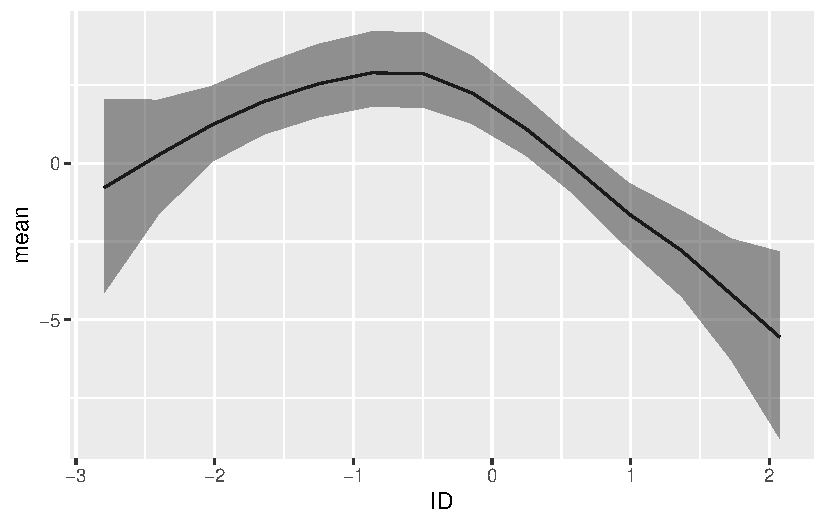
\includegraphics[keepaspectratio]{day3_practical_5_files/figure-pdf/unnamed-chunk-54-1.pdf}}

\begin{tcolorbox}[enhanced jigsaw, coltitle=black, bottomtitle=1mm, leftrule=.75mm, left=2mm, colback=white, colbacktitle=quarto-callout-warning-color!10!white, breakable, toptitle=1mm, titlerule=0mm, title={Task}, arc=.35mm, toprule=.15mm, bottomrule=.15mm, rightrule=.15mm, opacitybacktitle=0.6, opacityback=0, colframe=quarto-callout-warning-color-frame]

Create a map of predicted \emph{probability} from Model 3. You can use a
inverse logit function defined as

\begin{Shaded}
\begin{Highlighting}[]
\NormalTok{inv\_logit }\OtherTok{=} \ControlFlowTok{function}\NormalTok{(x) (}\DecValTok{1}\SpecialCharTok{+}\FunctionTok{exp}\NormalTok{(}\SpecialCharTok{{-}}\NormalTok{x))}\SpecialCharTok{\^{}}\NormalTok{(}\SpecialCharTok{{-}}\DecValTok{1}\NormalTok{)}
\end{Highlighting}
\end{Shaded}

Take hint

The \texttt{predict()} function can take as input also functions of
elements of the components you want to consider

Click here to see the solution

\begin{Shaded}
\begin{Highlighting}[]
\NormalTok{inv\_logit }\OtherTok{=} \ControlFlowTok{function}\NormalTok{(x) (}\DecValTok{1}\SpecialCharTok{+}\FunctionTok{exp}\NormalTok{(}\SpecialCharTok{{-}}\NormalTok{x))}\SpecialCharTok{\^{}}\NormalTok{(}\SpecialCharTok{{-}}\DecValTok{1}\NormalTok{)}

\NormalTok{pred3  }\OtherTok{=} \FunctionTok{predict}\NormalTok{(fit3, pxl1, }\SpecialCharTok{\textasciitilde{}}\FunctionTok{inv\_logit}\NormalTok{(Intercept }\SpecialCharTok{+}\NormalTok{ space }\SpecialCharTok{+}\NormalTok{ covariate) )}

\NormalTok{pred3 }\SpecialCharTok{\%\textgreater{}\%} \FunctionTok{ggplot}\NormalTok{() }\SpecialCharTok{+} 
      \FunctionTok{geom\_sf}\NormalTok{(}\FunctionTok{aes}\NormalTok{(}\AttributeTok{color =}\NormalTok{ mean)) }\SpecialCharTok{+}
        \FunctionTok{scale\_color\_scico}\NormalTok{(}\AttributeTok{direction =} \SpecialCharTok{{-}}\DecValTok{1}\NormalTok{) }\SpecialCharTok{+}
        \FunctionTok{ggtitle}\NormalTok{(}\StringTok{"Sample from the fitted model"}\NormalTok{)}
\end{Highlighting}
\end{Shaded}

\begin{center}
\pandocbounded{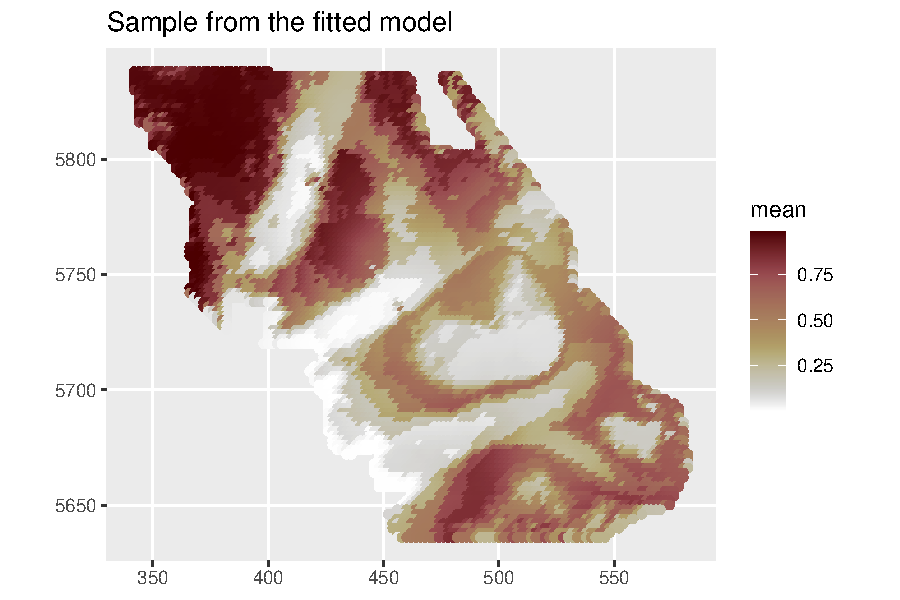
\includegraphics[keepaspectratio]{day3_practical_5_files/figure-pdf/unnamed-chunk-56-1.pdf}}
\end{center}

\end{tcolorbox}

\section{Log-Gaussian Cox Processes}\label{sec-linmodel}

In this practical we will:

\begin{itemize}
\tightlist
\item
  Fit a \hyperref[HPP]{homogeneous Point Process}
\item
  Fit a \hyperref[NHPP]{non-homogeneous Point Process}
\item
  Fit a \hyperref[LGCP]{LGCP (log-Gaussian Cox Process)}
\end{itemize}

Libraries to load:

\begin{Shaded}
\begin{Highlighting}[]
\FunctionTok{library}\NormalTok{(dplyr)}
\FunctionTok{library}\NormalTok{(INLA)}
\FunctionTok{library}\NormalTok{(ggplot2)}
\FunctionTok{library}\NormalTok{(patchwork)}
\FunctionTok{library}\NormalTok{(inlabru)     }
\FunctionTok{library}\NormalTok{(spatstat)}
\FunctionTok{library}\NormalTok{(sf)}
\FunctionTok{library}\NormalTok{(scico)}
\FunctionTok{library}\NormalTok{(spatstat)}
\FunctionTok{library}\NormalTok{(lubridate)}
\FunctionTok{library}\NormalTok{(terra)}
\FunctionTok{library}\NormalTok{(tidyterra)}
\end{Highlighting}
\end{Shaded}

\begin{center}\rule{0.5\linewidth}{0.5pt}\end{center}

\subsection{The data}\label{the-data-2}

In this practical we consider the data \texttt{clmfires} in the
\texttt{spatstat} library.

This dataset is a record of forest fires in the Castilla-La Mancha
region of Spain between 1998 and 2007. This region is approximately 400
by 400 kilometres. The coordinates are recorded in kilometres. For more
info about the data you can type:

\begin{Shaded}
\begin{Highlighting}[]
\NormalTok{?clmfires}
\end{Highlighting}
\end{Shaded}

We first read the data and transform them into an \texttt{sf} object. We
also create a polygon that represents the border of the Castilla-La
Mancha region. We select the data for year 2004 and only those fires
caused by lightning.

\begin{Shaded}
\begin{Highlighting}[]
\FunctionTok{data}\NormalTok{(}\StringTok{"clmfires"}\NormalTok{)}
\NormalTok{pp }\OtherTok{=} \FunctionTok{st\_as\_sf}\NormalTok{(}\FunctionTok{as.data.frame}\NormalTok{(clmfires) }\SpecialCharTok{\%\textgreater{}\%}
                \FunctionTok{mutate}\NormalTok{(}\AttributeTok{x =}\NormalTok{ x, }
                       \AttributeTok{y =}\NormalTok{ y),}
              \AttributeTok{coords =} \FunctionTok{c}\NormalTok{(}\StringTok{"x"}\NormalTok{,}\StringTok{"y"}\NormalTok{),}
              \AttributeTok{crs =} \ConstantTok{NA}\NormalTok{) }\SpecialCharTok{\%\textgreater{}\%}
  \FunctionTok{filter}\NormalTok{(cause }\SpecialCharTok{==} \StringTok{"lightning"}\NormalTok{,}
         \FunctionTok{year}\NormalTok{(date) }\SpecialCharTok{==} \DecValTok{2004}\NormalTok{)}

\NormalTok{poly }\OtherTok{=} \FunctionTok{as.data.frame}\NormalTok{(clmfires}\SpecialCharTok{$}\NormalTok{window}\SpecialCharTok{$}\NormalTok{bdry[[}\DecValTok{1}\NormalTok{]]) }\SpecialCharTok{\%\textgreater{}\%}
  \FunctionTok{mutate}\NormalTok{(}\AttributeTok{ID =} \DecValTok{1}\NormalTok{)}

\NormalTok{region }\OtherTok{=}\NormalTok{ poly }\SpecialCharTok{\%\textgreater{}\%} 
  \FunctionTok{st\_as\_sf}\NormalTok{(}\AttributeTok{coords =} \FunctionTok{c}\NormalTok{(}\StringTok{"x"}\NormalTok{, }\StringTok{"y"}\NormalTok{), }\AttributeTok{crs =} \ConstantTok{NA}\NormalTok{) }\SpecialCharTok{\%\textgreater{}\%} 
\NormalTok{  dplyr}\SpecialCharTok{::}\FunctionTok{group\_by}\NormalTok{(ID) }\SpecialCharTok{\%\textgreater{}\%} 
  \FunctionTok{summarise}\NormalTok{(}\AttributeTok{geometry =} \FunctionTok{st\_combine}\NormalTok{(geometry)) }\SpecialCharTok{\%\textgreater{}\%}
  \FunctionTok{st\_cast}\NormalTok{(}\StringTok{"POLYGON"}\NormalTok{) }
  
\FunctionTok{ggplot}\NormalTok{() }\SpecialCharTok{+} \FunctionTok{geom\_sf}\NormalTok{(}\AttributeTok{data =}\NormalTok{ region, }\AttributeTok{alpha =} \DecValTok{0}\NormalTok{) }\SpecialCharTok{+} \FunctionTok{geom\_sf}\NormalTok{(}\AttributeTok{data =}\NormalTok{ pp)  }
\end{Highlighting}
\end{Shaded}

\begin{figure}[H]

\centering{

\pandocbounded{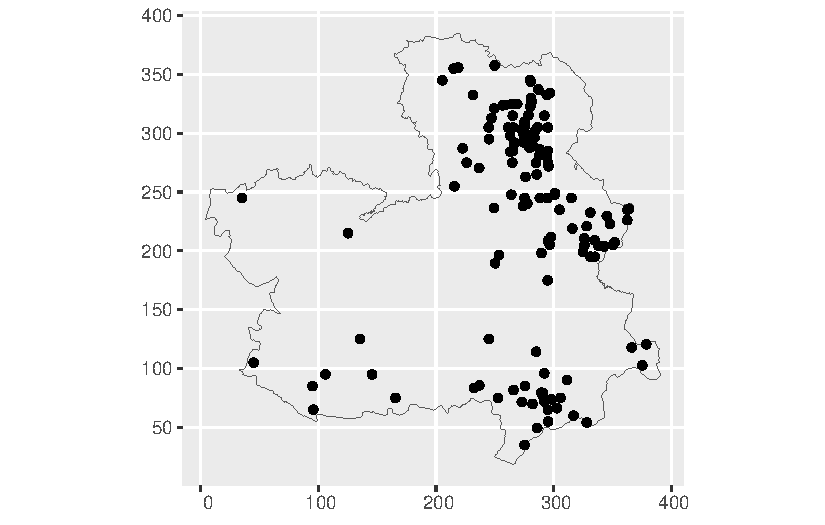
\includegraphics[keepaspectratio]{day3_practical_5_files/figure-pdf/fig-points-1.pdf}}

}

\caption{\label{fig-points}Distribution of the observed forest fires
caused by lightning in Castilla-La Mancha in 2004}

\end{figure}%

\subsection{Fit a homogeneous Poisson Process}\label{HPP}

As a first exercise we are going to fit a homogeneous Poisson process
(HPP) to the data. This is a model that assume constant intensity over
the whole space so our linear predictor is then:

\[
\eta(s) = \log\lambda(s) = \beta_0 , \ \mathbf{s}\in\Omega
\]

so the likelihood can be written as:

\[
\begin{aligned}
p(\mathbf{y} | \lambda)  & \propto \exp \left( -\int_\Omega \lambda(\mathbf{s}) \mathrm{d}\mathbf{s} \right) \prod_{i=1}^n \lambda(\mathbf{s}_i) \\
& = \exp\left( -\int_{\Omega}\exp(\beta_0)ds\right)\prod_{i=1}^n \lambda(\mathbf{s}_i) \\
\end{aligned}
\]

where \(|\Omega|\) is the area of the domain of interest.

We need to approximate the integral using a numerical integration scheme
as:

\[
\approx\exp\left(-\sum_{k=1}^{N_k}w_k\lambda(s_k)\right)\prod_{i=1}^n \lambda(\mathbf{s}_i)
\]

Where \(N_k\) is the number of integration points \(s_1,\dots,s_{N_k}\)
and \(w_1,\dots,w_{N_k}\) are the integration weights.

In this case, since the intensity is constant, the integration scheme is
really simple: it is enough to consider one random point inside the
domain with weight equal to the area of the domain.

\begin{Shaded}
\begin{Highlighting}[]
\CommentTok{\# define integration scheme}

\NormalTok{ips }\OtherTok{=} \FunctionTok{st\_sf}\NormalTok{(}
\AttributeTok{geometry =} \FunctionTok{st\_sample}\NormalTok{(region, }\DecValTok{1}\NormalTok{)) }\CommentTok{\# some random location inside the domain}
\NormalTok{ips}\SpecialCharTok{$}\NormalTok{weight }\OtherTok{=} \FunctionTok{st\_area}\NormalTok{(region) }\CommentTok{\# integration weight is the area of the domain}

\NormalTok{cmp }\OtherTok{=} \ErrorTok{\textasciitilde{}} \DecValTok{0} \SpecialCharTok{+} \FunctionTok{beta\_0}\NormalTok{(}\DecValTok{1}\NormalTok{)}

\NormalTok{formula }\OtherTok{=}\NormalTok{ geometry }\SpecialCharTok{\textasciitilde{}}\NormalTok{ beta\_0}

\NormalTok{lik }\OtherTok{=} \FunctionTok{bru\_obs}\NormalTok{(}\AttributeTok{data =}\NormalTok{ pp,}
              \AttributeTok{family =} \StringTok{"cp"}\NormalTok{,}
              \AttributeTok{formula =}\NormalTok{ formula,}
              \AttributeTok{ips =}\NormalTok{ ips)}
\NormalTok{fit1 }\OtherTok{=} \FunctionTok{bru}\NormalTok{(cmp, lik)}
\end{Highlighting}
\end{Shaded}

\begin{tcolorbox}[enhanced jigsaw, coltitle=black, bottomtitle=1mm, leftrule=.75mm, left=2mm, colback=white, colbacktitle=quarto-callout-warning-color!10!white, breakable, toptitle=1mm, titlerule=0mm, title={Task}, arc=.35mm, toprule=.15mm, bottomrule=.15mm, rightrule=.15mm, opacitybacktitle=0.6, opacityback=0, colframe=quarto-callout-warning-color-frame]

\begin{enumerate}
\def\labelenumi{\arabic{enumi}.}
\tightlist
\item
  Plot the estimated posterior distribution of the intensity
\item
  Compare the estimated expected number of fires on the whole domain
  with the observed ones.
\end{enumerate}

Take hint

Remember that in the \emph{inlabru} framework we model the log intensity
\(\eta = log(\lambda)\)

Click here to see the solution

\begin{Shaded}
\begin{Highlighting}[]
\CommentTok{\# 1) The estimated posterior distribution of the  intensity is}

\NormalTok{post\_int }\OtherTok{=} \FunctionTok{inla.tmarginal}\NormalTok{(}\ControlFlowTok{function}\NormalTok{(x) }\FunctionTok{exp}\NormalTok{(x), fit1}\SpecialCharTok{$}\NormalTok{marginals.fixed}\SpecialCharTok{$}\NormalTok{beta\_0)}
\NormalTok{post\_int }\SpecialCharTok{\%\textgreater{}\%} \FunctionTok{ggplot}\NormalTok{() }\SpecialCharTok{+} \FunctionTok{geom\_line}\NormalTok{(}\FunctionTok{aes}\NormalTok{(x,y))}
\end{Highlighting}
\end{Shaded}

\begin{center}
\pandocbounded{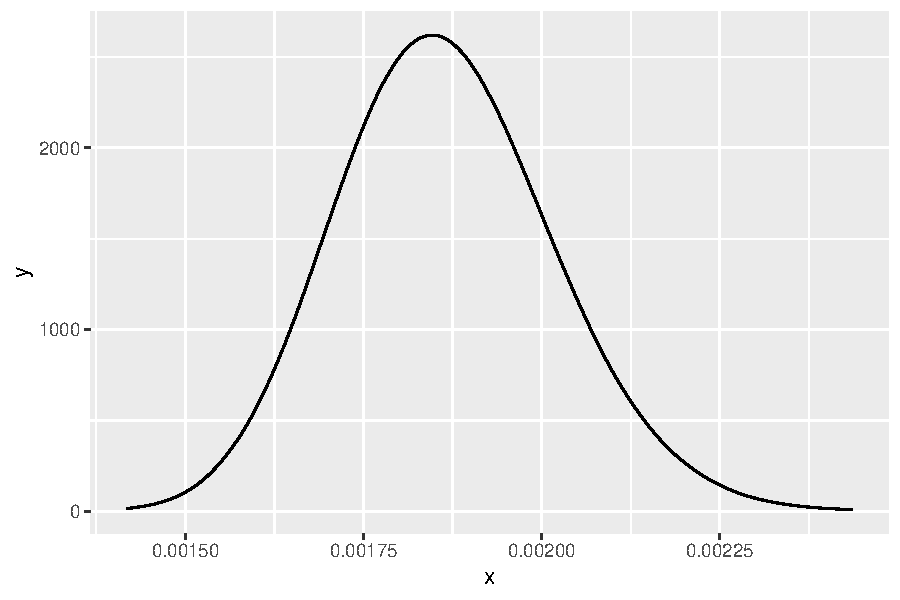
\includegraphics[keepaspectratio]{day3_practical_5_files/figure-pdf/unnamed-chunk-91-1.pdf}}
\end{center}

\begin{Shaded}
\begin{Highlighting}[]
\CommentTok{\# 2) To compute the expected number of points in the area we need to multiply the}
\CommentTok{\# estimated intensity by the area of the domain.}
\CommentTok{\# In the same plot we also show the number of observed fires as a vertical line.}

\NormalTok{post\_int }\OtherTok{=} \FunctionTok{inla.tmarginal}\NormalTok{(}\ControlFlowTok{function}\NormalTok{(x) }\FunctionTok{st\_area}\NormalTok{(region)}\SpecialCharTok{*} \FunctionTok{exp}\NormalTok{(x), fit1}\SpecialCharTok{$}\NormalTok{marginals.fixed}\SpecialCharTok{$}\NormalTok{beta\_0)}
\NormalTok{post\_int }\SpecialCharTok{\%\textgreater{}\%} \FunctionTok{ggplot}\NormalTok{() }\SpecialCharTok{+} \FunctionTok{geom\_line}\NormalTok{(}\FunctionTok{aes}\NormalTok{(x,y)) }\SpecialCharTok{+}
  \FunctionTok{geom\_vline}\NormalTok{(}\AttributeTok{xintercept =} \FunctionTok{dim}\NormalTok{(pp)[}\DecValTok{1}\NormalTok{])}
\end{Highlighting}
\end{Shaded}

\begin{center}
\pandocbounded{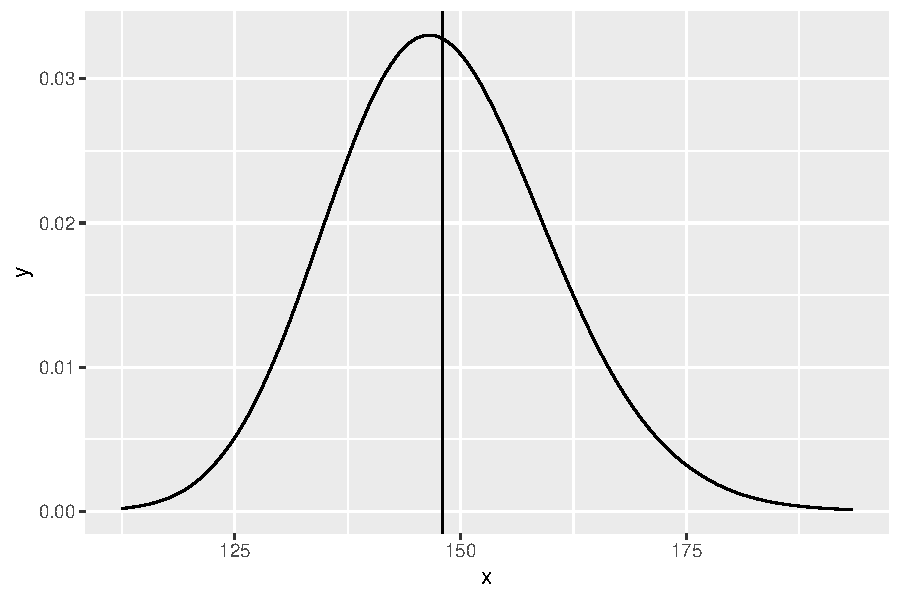
\includegraphics[keepaspectratio]{day3_practical_5_files/figure-pdf/unnamed-chunk-91-2.pdf}}
\end{center}

\end{tcolorbox}

\subsection{Fit an Inhomogeneous Poisson Process}\label{NHPP}

The model above has the clear disadvantages that assumes a constant
intensity and from Figure~\ref{fig-points} we clearly see that this is
not the case.

The library \texttt{spatstat} contains also some covariates that can
help explain the fires distribution. Figure @fit-altitude shows the
location of fires together with the (scaled) altitude.

\begin{Shaded}
\begin{Highlighting}[]
\CommentTok{\#|label: fig{-}altitude}
\CommentTok{\#|fig{-}cap: "Distribution of the observed forest fires and scaled altitude"}
\CommentTok{\#| }
\NormalTok{elev\_raster }\OtherTok{=} \FunctionTok{rast}\NormalTok{(clmfires.extra[[}\DecValTok{2}\NormalTok{]]}\SpecialCharTok{$}\NormalTok{elevation)}
\NormalTok{elev\_raster }\OtherTok{=} \FunctionTok{scale}\NormalTok{(elev\_raster)}
\FunctionTok{ggplot}\NormalTok{() }\SpecialCharTok{+} 
  \FunctionTok{geom\_spatraster}\NormalTok{(}\AttributeTok{data =}\NormalTok{ elev\_raster) }\SpecialCharTok{+} 
  \FunctionTok{geom\_sf}\NormalTok{(}\AttributeTok{data =}\NormalTok{ pp) }\SpecialCharTok{+}
  \FunctionTok{scale\_fill\_scico}\NormalTok{()}
\end{Highlighting}
\end{Shaded}

\pandocbounded{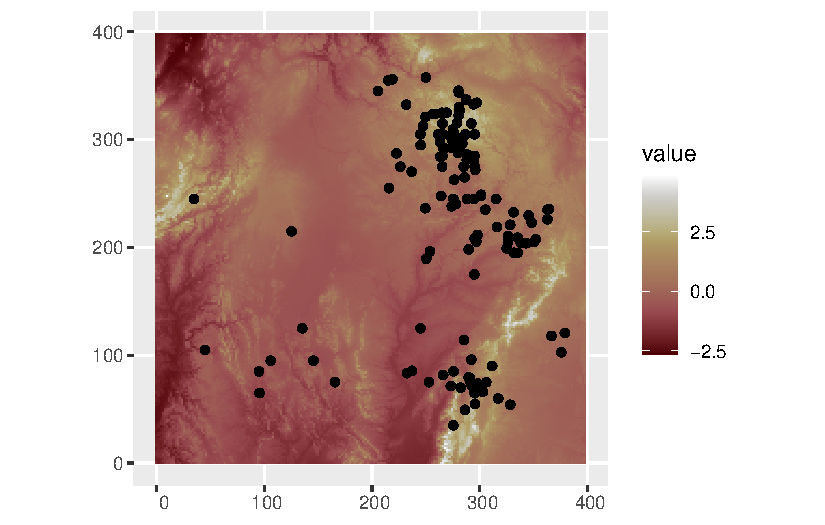
\includegraphics[keepaspectratio]{day3_practical_5_files/figure-pdf/unnamed-chunk-92-1.pdf}}

We are now going to use the altitude as a covariate to explain the
variability of the intensity \(\lambda(s)\) over the domain of interest.

Our model is \[
\log\lambda(s) = \beta_0 + \beta_1x(s)
\] where \(x(s)\) is the altitude at location \(s\).

The likelihood becomes:

\[
\begin{aligned}
p(\mathbf{y} | \lambda)  & \propto \exp \left( -\int_\Omega \lambda(\mathbf{s}) \mathrm{d}\mathbf{s} \right) \prod_{i=1}^n \lambda(\mathbf{s}_i) \\
& = \exp \left( -\int_\Omega \exp(\beta_0 + \beta_1x(s)) \mathrm{d}\mathbf{s} \right) \prod_{i=1}^n \lambda(\mathbf{s}_i) \\
\end{aligned}
\]

Now we need to choose an integration scheme to solve the integral.

In this case we will take a simple grid based approach where each
quadrature location has an equal weight. Our grid consists of
\(N_k = 1000\) points and the weights are all equal to \(|\Omega|/N_k\).

\begin{Shaded}
\begin{Highlighting}[]
\CommentTok{\#|label: fig{-}int2}
\CommentTok{\#|fig{-}cap: "Integration scheme."}

\NormalTok{n.int }\OtherTok{=} \DecValTok{1000}
\NormalTok{ips }\OtherTok{=} \FunctionTok{st\_sf}\NormalTok{(}\AttributeTok{geometry =} \FunctionTok{st\_sample}\NormalTok{(region,}
            \AttributeTok{size =}\NormalTok{ n.int,}
            \AttributeTok{type =} \StringTok{"regular"}\NormalTok{))}

\NormalTok{ips}\SpecialCharTok{$}\NormalTok{weight }\OtherTok{=} \FunctionTok{st\_area}\NormalTok{(region) }\SpecialCharTok{/}\NormalTok{ n.int}
\FunctionTok{ggplot}\NormalTok{() }\SpecialCharTok{+} \FunctionTok{geom\_sf}\NormalTok{(}\AttributeTok{data =}\NormalTok{ ips, }\FunctionTok{aes}\NormalTok{(}\AttributeTok{color =}\NormalTok{ weight)) }\SpecialCharTok{+} \FunctionTok{geom\_sf}\NormalTok{(}\AttributeTok{data=}\NormalTok{ region, }\AttributeTok{alpha =} \DecValTok{0}\NormalTok{)}
\end{Highlighting}
\end{Shaded}

\pandocbounded{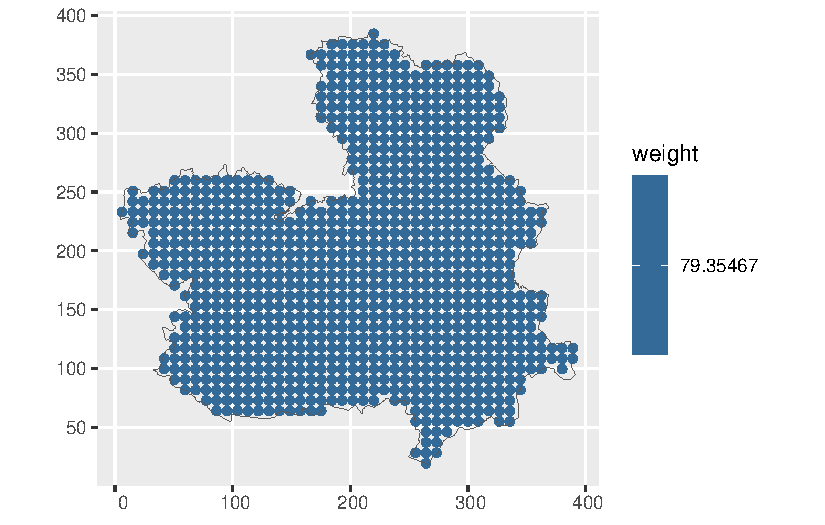
\includegraphics[keepaspectratio]{day3_practical_5_files/figure-pdf/unnamed-chunk-93-1.pdf}}

\textbf{OBS}: The implicit assumption here is that the intensity is
constant inside each grid box, \emph{and so is the covariate}!!

We can now fit the model:

\begin{Shaded}
\begin{Highlighting}[]
\NormalTok{cmp }\OtherTok{=} \ErrorTok{\textasciitilde{}} \FunctionTok{Intercept}\NormalTok{(}\DecValTok{1}\NormalTok{) }\SpecialCharTok{+} \FunctionTok{elev}\NormalTok{(elev\_raster, }\AttributeTok{model =} \StringTok{"linear"}\NormalTok{)}
\NormalTok{formula }\OtherTok{=}\NormalTok{ geometry }\SpecialCharTok{\textasciitilde{}}\NormalTok{ Intercept }\SpecialCharTok{+}\NormalTok{ elev}
\NormalTok{lik }\OtherTok{=} \FunctionTok{bru\_obs}\NormalTok{(}\AttributeTok{data =}\NormalTok{ pp,}
              \AttributeTok{family =} \StringTok{"cp"}\NormalTok{,}
              \AttributeTok{formula =}\NormalTok{ formula,}
              \AttributeTok{ips =}\NormalTok{ ips)}
\NormalTok{fit2 }\OtherTok{=} \FunctionTok{bru}\NormalTok{(cmp, lik)}
\end{Highlighting}
\end{Shaded}

\begin{tcolorbox}[enhanced jigsaw, coltitle=black, bottomtitle=1mm, leftrule=.75mm, left=2mm, colback=white, colbacktitle=quarto-callout-warning-color!10!white, breakable, toptitle=1mm, titlerule=0mm, title={Task}, arc=.35mm, toprule=.15mm, bottomrule=.15mm, rightrule=.15mm, opacitybacktitle=0.6, opacityback=0, colframe=quarto-callout-warning-color-frame]

What is the effect of the altitude on the (log) intensity of the
process?

Take hint

You can look at the summary for the fixed effects

Click here to see the solution

\begin{Shaded}
\begin{Highlighting}[]
\NormalTok{fit2}\SpecialCharTok{$}\NormalTok{summary.fixed}
\end{Highlighting}
\end{Shaded}

\begin{verbatim}
                mean         sd 0.025quant   0.5quant 0.975quant       mode kld
Intercept -6.6212999 0.10325267  -6.823671 -6.6212999 -6.4189284 -6.6212999   0
elev       0.6773998 0.07187518   0.536527  0.6773998  0.8182726  0.6773998   0
\end{verbatim}

\end{tcolorbox}

\begin{tcolorbox}[enhanced jigsaw, coltitle=black, bottomtitle=1mm, leftrule=.75mm, left=2mm, colback=white, colbacktitle=quarto-callout-warning-color!10!white, breakable, toptitle=1mm, titlerule=0mm, title=\textcolor{quarto-callout-warning-color}{\faExclamationTriangle}\hspace{0.5em}{Warning}, arc=.35mm, toprule=.15mm, bottomrule=.15mm, rightrule=.15mm, opacitybacktitle=0.6, opacityback=0, colframe=quarto-callout-warning-color-frame]

⚠️ \textbf{WARNING!!}⚠️ When fitting a Point process, the integration
scheme has to be fine enough to capture the spatial variability of the
covariate!!

\end{tcolorbox}

\begin{tcolorbox}[enhanced jigsaw, coltitle=black, bottomtitle=1mm, leftrule=.75mm, left=2mm, colback=white, colbacktitle=quarto-callout-warning-color!10!white, breakable, toptitle=1mm, titlerule=0mm, title={Task}, arc=.35mm, toprule=.15mm, bottomrule=.15mm, rightrule=.15mm, opacitybacktitle=0.6, opacityback=0, colframe=quarto-callout-warning-color-frame]

Rerun the model with the altitude as covariate, but this time change the
integration scheme as follows:

\begin{Shaded}
\begin{Highlighting}[]
\NormalTok{n.int2 }\OtherTok{=} \DecValTok{50}

\NormalTok{ips2 }\OtherTok{=} \FunctionTok{st\_sf}\NormalTok{(}\AttributeTok{geometry =} \FunctionTok{st\_sample}\NormalTok{(region,}
            \AttributeTok{size =}\NormalTok{ n.int2,}
            \AttributeTok{type =} \StringTok{"regular"}\NormalTok{))}
\NormalTok{ips2}\SpecialCharTok{$}\NormalTok{weight }\OtherTok{=} \FunctionTok{st\_area}\NormalTok{(region) }\SpecialCharTok{/}\NormalTok{ n.int2}
\end{Highlighting}
\end{Shaded}

What happens to the effect of the covariate?

Take hint

Re-run the model changing the integration scheme in the \emph{ips} input
of the \emph{bru\_obs()} function.

Click here to see the solution

\begin{Shaded}
\begin{Highlighting}[]
\NormalTok{lik\_bis }\OtherTok{=} \FunctionTok{bru\_obs}\NormalTok{(}\AttributeTok{data =}\NormalTok{ pp,}
              \AttributeTok{family =} \StringTok{"cp"}\NormalTok{,}
              \AttributeTok{formula =}\NormalTok{ formula,}
              \AttributeTok{ips =}\NormalTok{ ips2)}

\NormalTok{fit2bis }\OtherTok{=} \FunctionTok{bru}\NormalTok{(cmp, lik\_bis)}

\CommentTok{\# you can the check the differences between the two models}
\FunctionTok{rbind}\NormalTok{(fit2}\SpecialCharTok{$}\NormalTok{summary.fixed,}
\NormalTok{fit2bis}\SpecialCharTok{$}\NormalTok{summary.fixed)}
\end{Highlighting}
\end{Shaded}

\begin{verbatim}
                 mean         sd 0.025quant   0.5quant 0.975quant       mode
Intercept  -6.6212999 0.10325267  -6.823671 -6.6212999 -6.4189284 -6.6212999
elev        0.6773998 0.07187518   0.536527  0.6773998  0.8182726  0.6773998
Intercept1 -6.4112966 0.09479277  -6.597087 -6.4112966 -6.2255062 -6.4112966
elev1       0.4411505 0.05430789   0.334709  0.4411505  0.5475920  0.4411505
           kld
Intercept    0
elev         0
Intercept1   0
elev1        0
\end{verbatim}

\end{tcolorbox}

\begin{tcolorbox}[enhanced jigsaw, coltitle=black, bottomtitle=1mm, leftrule=.75mm, left=2mm, colback=white, colbacktitle=quarto-callout-warning-color!10!white, breakable, toptitle=1mm, titlerule=0mm, title={Task}, arc=.35mm, toprule=.15mm, bottomrule=.15mm, rightrule=.15mm, opacitybacktitle=0.6, opacityback=0, colframe=quarto-callout-warning-color-frame]

Now we want to predict the log-intensity over the whole domain. Use the
grid from the elevation raster to predict the intensity over the domain.

\begin{Shaded}
\begin{Highlighting}[]
\NormalTok{est\_grid }\OtherTok{=} \FunctionTok{st\_as\_sf}\NormalTok{(}\FunctionTok{data.frame}\NormalTok{(}\FunctionTok{crds}\NormalTok{(elev\_raster)), }\AttributeTok{coords =} \FunctionTok{c}\NormalTok{(}\StringTok{"x"}\NormalTok{,}\StringTok{"y"}\NormalTok{))}
\NormalTok{est\_grid  }\OtherTok{=} \FunctionTok{st\_intersection}\NormalTok{(est\_grid, region)}
\end{Highlighting}
\end{Shaded}

Click here to see the solution

\begin{Shaded}
\begin{Highlighting}[]
\NormalTok{preds2 }\OtherTok{=} \FunctionTok{predict}\NormalTok{(fit2, est\_grid, }\SpecialCharTok{\textasciitilde{}} \FunctionTok{data.frame}\NormalTok{(}\AttributeTok{log\_scale =}\NormalTok{ Intercept }\SpecialCharTok{+}\NormalTok{ elev,}

                                              \AttributeTok{lin\_scale =} \FunctionTok{exp}\NormalTok{(Intercept }\SpecialCharTok{+}\NormalTok{ elev)))}
\CommentTok{\# then visualize it like}
\NormalTok{preds2}\SpecialCharTok{$}\NormalTok{log\_scale }\SpecialCharTok{\%\textgreater{}\%} 
  \FunctionTok{ggplot}\NormalTok{() }\SpecialCharTok{+}
  \FunctionTok{geom\_sf}\NormalTok{(}\FunctionTok{aes}\NormalTok{(}\AttributeTok{color =}\NormalTok{ mean)) }\SpecialCharTok{+}
  \FunctionTok{scale\_color\_scico}\NormalTok{()}
\end{Highlighting}
\end{Shaded}

\begin{center}
\pandocbounded{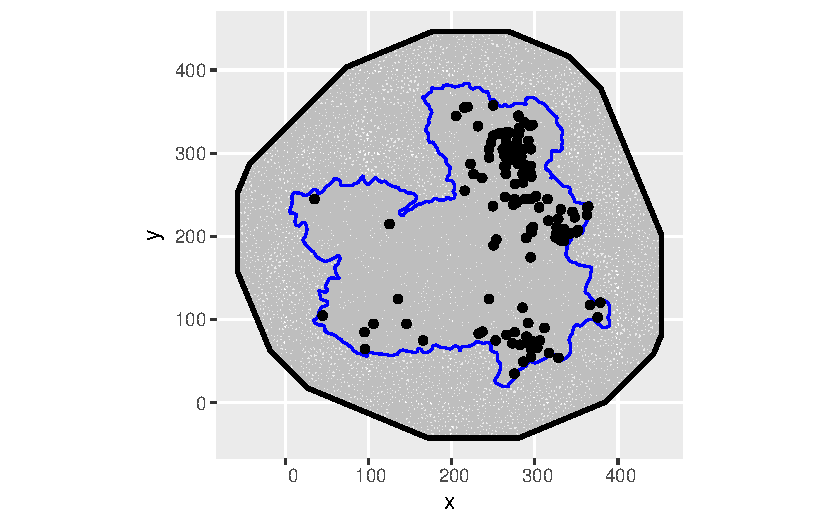
\includegraphics[keepaspectratio]{day3_practical_5_files/figure-pdf/unnamed-chunk-99-1.pdf}}
\end{center}

\end{tcolorbox}

Finally, we want to use the fitted model to estimate the total number of
fires over the whole region. To do this we first have to fine the
expected number of fires as:

\[
E(N_{\Omega}) = \int_{\Omega}\exp(\lambda(s))\ ds
\]

Then simulate possible realizations of \(N_{\Omega}\) to include also
the likelihood variability in our estimate:

\begin{Shaded}
\begin{Highlighting}[]
\NormalTok{N\_fires }\OtherTok{=} \FunctionTok{generate}\NormalTok{(fit2, ips,}
                      \AttributeTok{formula =} \SpecialCharTok{\textasciitilde{}}\NormalTok{ \{}
\NormalTok{                        lambda }\OtherTok{=} \FunctionTok{sum}\NormalTok{(weight }\SpecialCharTok{*} \FunctionTok{exp}\NormalTok{(elev }\SpecialCharTok{+}\NormalTok{ Intercept))}
                        \FunctionTok{rpois}\NormalTok{(}\DecValTok{1}\NormalTok{, lambda)\},}
                    \AttributeTok{n.samples =} \DecValTok{2000}\NormalTok{)}

\FunctionTok{ggplot}\NormalTok{(}\AttributeTok{data =} \FunctionTok{data.frame}\NormalTok{(}\AttributeTok{N =} \FunctionTok{as.vector}\NormalTok{(N\_fires))) }\SpecialCharTok{+}
  \FunctionTok{geom\_histogram}\NormalTok{(}\FunctionTok{aes}\NormalTok{(}\AttributeTok{x =}\NormalTok{ N),}
                 \AttributeTok{colour =} \StringTok{"blue"}\NormalTok{,}
                 \AttributeTok{alpha =} \FloatTok{0.5}\NormalTok{,}
                 \AttributeTok{bins =} \DecValTok{20}\NormalTok{) }\SpecialCharTok{+}
  \FunctionTok{geom\_vline}\NormalTok{(}\AttributeTok{xintercept =} \FunctionTok{nrow}\NormalTok{(pp),}
             \AttributeTok{colour =} \StringTok{"red"}\NormalTok{) }\SpecialCharTok{+}
  \FunctionTok{theme\_minimal}\NormalTok{() }\SpecialCharTok{+}
  \FunctionTok{xlab}\NormalTok{(}\FunctionTok{expression}\NormalTok{(Lambda))}
\end{Highlighting}
\end{Shaded}

\pandocbounded{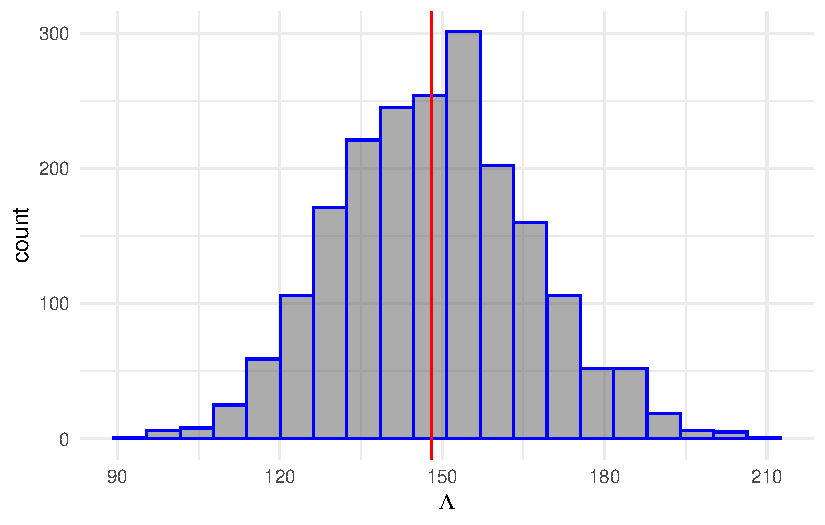
\includegraphics[keepaspectratio]{day3_practical_5_files/figure-pdf/unnamed-chunk-100-1.pdf}}

\subsection{Fit a Log-Gaussian Cox Process}\label{LGCP}

Finally we want to fit a LGCP with log intensity:

\[
\log(s) = \beta_0 + \beta_1x + u(s)
\]

where \(\beta_0\) is the intercept, \(\beta_1\) the effect of
(standarized) altitude \(x(s)\) as before and \(u(s)\) is a Gaussian
Random field defined through the SPDE approach.

\subsubsection{Define the mesh}\label{define-the-mesh}

The first step, as any time we use the SPDE approach is to defie the
mesh and the priors for the marginal variance and range:

\begin{Shaded}
\begin{Highlighting}[]
\NormalTok{mesh }\OtherTok{=} \FunctionTok{fm\_mesh\_2d}\NormalTok{(}\AttributeTok{boundary =}\NormalTok{ region,}
                  \AttributeTok{max.edge =} \FunctionTok{c}\NormalTok{(}\DecValTok{5}\NormalTok{, }\DecValTok{10}\NormalTok{),}
                  \AttributeTok{cutoff =} \DecValTok{4}\NormalTok{, }\AttributeTok{crs =} \ConstantTok{NA}\NormalTok{)}

\FunctionTok{ggplot}\NormalTok{() }\SpecialCharTok{+} \FunctionTok{gg}\NormalTok{(mesh) }\SpecialCharTok{+} \FunctionTok{geom\_sf}\NormalTok{(}\AttributeTok{data =}\NormalTok{ pp)}
\end{Highlighting}
\end{Shaded}

\pandocbounded{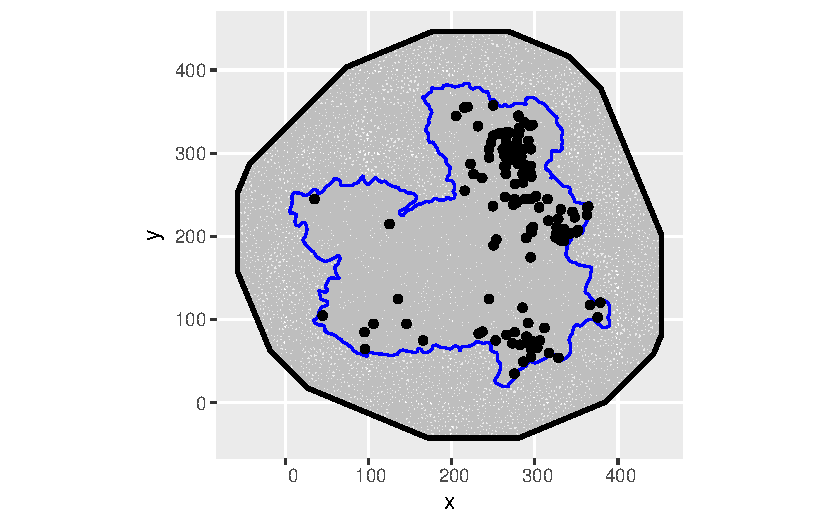
\includegraphics[keepaspectratio]{day3_practical_5_files/figure-pdf/unnamed-chunk-101-1.pdf}}

\begin{Shaded}
\begin{Highlighting}[]
\NormalTok{spde\_model }\OtherTok{=}  \FunctionTok{inla.spde2.pcmatern}\NormalTok{(mesh,}
                                  \AttributeTok{prior.sigma =} \FunctionTok{c}\NormalTok{(}\DecValTok{1}\NormalTok{, }\FloatTok{0.5}\NormalTok{),}
                                  \AttributeTok{prior.range =} \FunctionTok{c}\NormalTok{(}\DecValTok{100}\NormalTok{, }\FloatTok{0.5}\NormalTok{))}
\end{Highlighting}
\end{Shaded}

We can then define the integration weight. Here we use the same points
to \texttt{define\ the\ SPDE\ approximation} and to
\texttt{approximate\ the\ integral} in the likelihood. We will see later
that this does not have to be like this, BUT integration weight and SPDE
weights have to be consistent with each other!

\begin{Shaded}
\begin{Highlighting}[]
\NormalTok{ips }\OtherTok{=} \FunctionTok{fm\_int}\NormalTok{(mesh, }\AttributeTok{samplers =}\NormalTok{ region)}

\FunctionTok{ggplot}\NormalTok{() }\SpecialCharTok{+} \FunctionTok{geom\_sf}\NormalTok{(}\AttributeTok{data =}\NormalTok{ ips, }\FunctionTok{aes}\NormalTok{(}\AttributeTok{color =}\NormalTok{ weight)) }\SpecialCharTok{+}
  \FunctionTok{gg}\NormalTok{(mesh) }\SpecialCharTok{+}
   \FunctionTok{scale\_color\_scico}\NormalTok{()}
\end{Highlighting}
\end{Shaded}

\pandocbounded{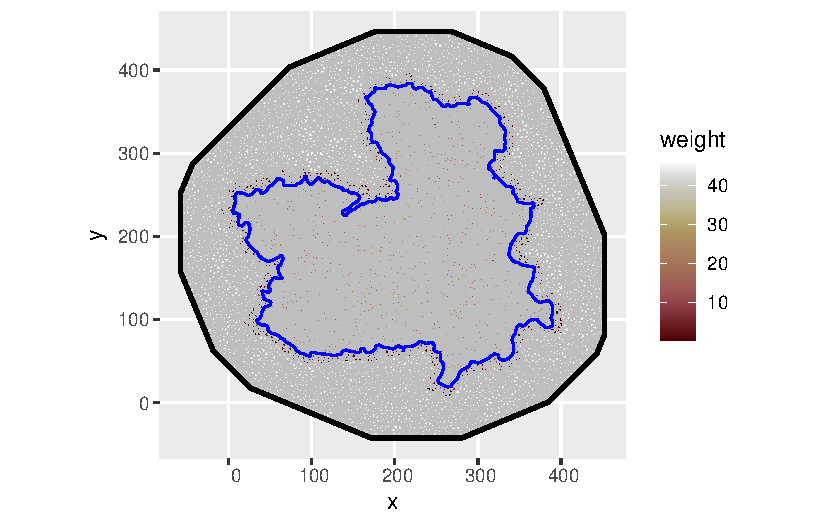
\includegraphics[keepaspectratio]{day3_practical_5_files/figure-pdf/unnamed-chunk-102-1.pdf}}

\subsubsection{Run the model}\label{run-the-model-1}

\begin{tcolorbox}[enhanced jigsaw, coltitle=black, bottomtitle=1mm, leftrule=.75mm, left=2mm, colback=white, colbacktitle=quarto-callout-warning-color!10!white, breakable, toptitle=1mm, titlerule=0mm, title={Task}, arc=.35mm, toprule=.15mm, bottomrule=.15mm, rightrule=.15mm, opacitybacktitle=0.6, opacityback=0, colframe=quarto-callout-warning-color-frame]

Set up the components and the formula for the model above by completing
the code below and run the model.

\begin{Shaded}
\begin{Highlighting}[]
\NormalTok{cmp }\OtherTok{=} \ErrorTok{\textasciitilde{}}\NormalTok{ ...}

\NormalTok{formula }\OtherTok{=}\NormalTok{ geometry }\SpecialCharTok{\textasciitilde{}}\NormalTok{ ...}

\NormalTok{lik }\OtherTok{=} \FunctionTok{bru\_obs}\NormalTok{(}\StringTok{"cp"}\NormalTok{,}
              \AttributeTok{formula =}\NormalTok{ formula,}
              \AttributeTok{data =}\NormalTok{ pp,}
              \AttributeTok{ips =}\NormalTok{ ...)}

\NormalTok{fit3 }\OtherTok{=} \FunctionTok{bru}\NormalTok{(cmp, lik)}
\end{Highlighting}
\end{Shaded}

Take hint

The model has three components: intercept, linear effect of altitude and
the spatial GRF

Click here to see the solution

\begin{Shaded}
\begin{Highlighting}[]
\NormalTok{cmp }\OtherTok{=} \ErrorTok{\textasciitilde{}} \FunctionTok{Intercept}\NormalTok{(}\DecValTok{1}\NormalTok{) }\SpecialCharTok{+} \FunctionTok{space}\NormalTok{(geometry, }\AttributeTok{model =}\NormalTok{ spde\_model) }\SpecialCharTok{+} \FunctionTok{elev}\NormalTok{(elev\_raster, }\AttributeTok{model =} \StringTok{"linear"}\NormalTok{)}

\NormalTok{formula }\OtherTok{=}\NormalTok{ geometry }\SpecialCharTok{\textasciitilde{}}\NormalTok{ Intercept }\SpecialCharTok{+}\NormalTok{ space }\SpecialCharTok{+}\NormalTok{ elev}

\NormalTok{lik }\OtherTok{=} \FunctionTok{bru\_obs}\NormalTok{(}\StringTok{"cp"}\NormalTok{,}
              \AttributeTok{formula =}\NormalTok{ formula,}
              \AttributeTok{data =}\NormalTok{ pp,}
              \AttributeTok{ips =}\NormalTok{ ips)}

\NormalTok{fit3 }\OtherTok{=} \FunctionTok{bru}\NormalTok{(cmp, lik)}
\end{Highlighting}
\end{Shaded}

\end{tcolorbox}

\textbf{Note} when running the model above you will get a warning:

\begin{verbatim}
Warning in bru_log_warn(msg): Model input 'elev_raster' for 'elev' returned some NA values.
Attempting to fill in spatially by nearest available value.
To avoid this basic covariate imputation, supply complete data.
\end{verbatim}

It means that the \emph{bru()} function cannot find the covariate values
for some of the mesh nodes. This is a common situation. As the warning
says, the \emph{bru()} function automatically imputes the value of the
covarite using the nearest nodes. This increases the running time of the
\emph{bru()} function, so one solution is to impute the values of the
covariate over the whole mesh `before' running the \emph{bru()}
function.

Here, we notice that there is a single point for which elevation values
are missing (see Figure~\ref{fig-points2} the red point that lies
outside the raster extension ).

\begin{figure}

\centering{

\pandocbounded{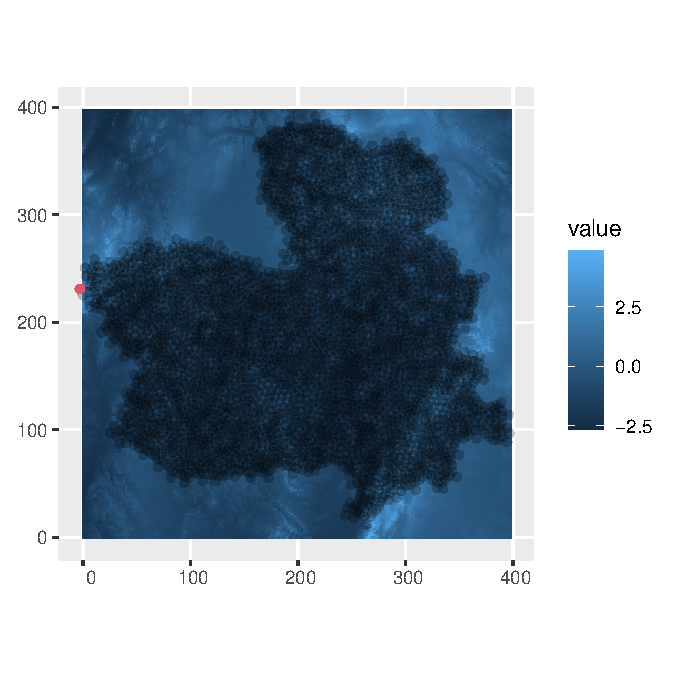
\includegraphics[keepaspectratio]{day3_practical_5_files/figure-pdf/fig-points2-1.pdf}}

}

\caption{\label{fig-points2}Integration scheme for numerical
approximation of the stochastic integral in La Mancha Region}

\end{figure}%

To solve this, we can increase the raster extension so it covers all
both data-points and quadrature locations as well. Then, we can use the
\texttt{bru\_fill\_missing()} function to input the missing values with
the nearest-available-value. We can achieve this using the following
code:

\begin{Shaded}
\begin{Highlighting}[]
\CommentTok{\# Extend raster ext by 30 \% of the original raster so it covers the whole mesh}
\NormalTok{re }\OtherTok{\textless{}{-}} \FunctionTok{extend}\NormalTok{(elev\_raster, }\FunctionTok{ext}\NormalTok{(elev\_raster)}\SpecialCharTok{*}\FloatTok{1.3}\NormalTok{)}
\CommentTok{\# Convert to an sf spatial object}
\NormalTok{re\_df }\OtherTok{\textless{}{-}}\NormalTok{ re }\SpecialCharTok{\%\textgreater{}\%}\NormalTok{ stars}\SpecialCharTok{::}\FunctionTok{st\_as\_stars}\NormalTok{() }\SpecialCharTok{\%\textgreater{}\%}  \FunctionTok{st\_as\_sf}\NormalTok{(}\AttributeTok{na.rm=}\NormalTok{F)}
\CommentTok{\# fill in missing values using the original raster }
\NormalTok{re\_df}\SpecialCharTok{$}\NormalTok{lyr}\FloatTok{.1} \OtherTok{\textless{}{-}} \FunctionTok{bru\_fill\_missing}\NormalTok{(elev\_raster,re\_df,re\_df}\SpecialCharTok{$}\NormalTok{lyr}\FloatTok{.1}\NormalTok{)}
\CommentTok{\# rasterize}
\NormalTok{elev\_rast\_p }\OtherTok{\textless{}{-}}\NormalTok{ stars}\SpecialCharTok{::}\FunctionTok{st\_rasterize}\NormalTok{(re\_df) }\SpecialCharTok{\%\textgreater{}\%} \FunctionTok{rast}\NormalTok{()}
\FunctionTok{ggplot}\NormalTok{() }\SpecialCharTok{+} \FunctionTok{geom\_spatraster}\NormalTok{(}\AttributeTok{data =}\NormalTok{ elev\_rast\_p) }
\end{Highlighting}
\end{Shaded}

\begin{center}
\pandocbounded{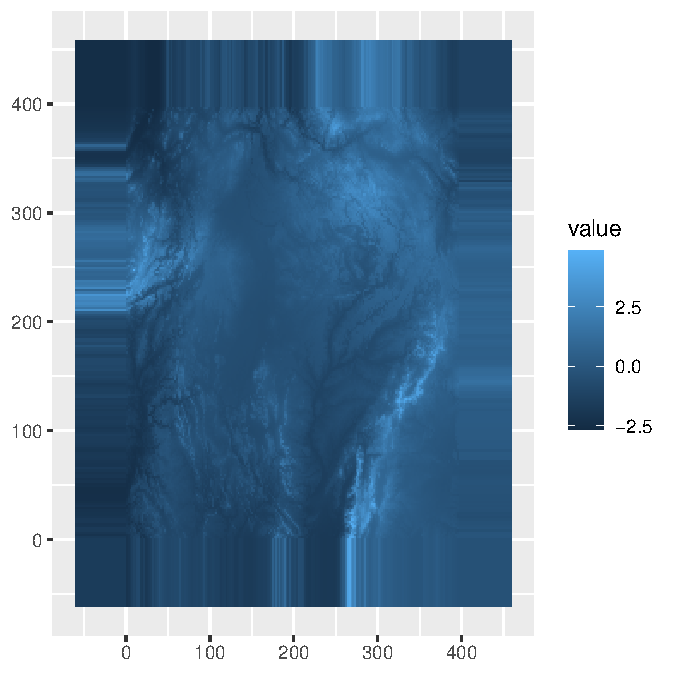
\includegraphics[keepaspectratio]{day3_practical_5_files/figure-pdf/unnamed-chunk-106-1.pdf}}
\end{center}

\begin{tcolorbox}[enhanced jigsaw, coltitle=black, bottomtitle=1mm, leftrule=.75mm, left=2mm, colback=white, colbacktitle=quarto-callout-note-color!10!white, breakable, toptitle=1mm, titlerule=0mm, title=\textcolor{quarto-callout-note-color}{\faInfo}\hspace{0.5em}{Note}, arc=.35mm, toprule=.15mm, bottomrule=.15mm, rightrule=.15mm, opacitybacktitle=0.6, opacityback=0, colframe=quarto-callout-note-color-frame]

The \texttt{bru\_fill\_missing()} function was added mainly to handle
very local infilling on domain boundaries. For properly missing data,
one should consider doing a proper model of the spatial field instead.

\end{tcolorbox}

\subsection{Results}\label{results}

\begin{tcolorbox}[enhanced jigsaw, coltitle=black, bottomtitle=1mm, leftrule=.75mm, left=2mm, colback=white, colbacktitle=quarto-callout-warning-color!10!white, breakable, toptitle=1mm, titlerule=0mm, title={Task}, arc=.35mm, toprule=.15mm, bottomrule=.15mm, rightrule=.15mm, opacitybacktitle=0.6, opacityback=0, colframe=quarto-callout-warning-color-frame]

Plot the estimated mean and standard deviation of the spatial GF and the
log-intensity over the domain of interest

Take hint

Use the \emph{fm\_pixels()} and \emph{predict()} functions.

Click here to see the solution

\begin{Shaded}
\begin{Highlighting}[]
\NormalTok{pxl }\OtherTok{=} \FunctionTok{fm\_pixels}\NormalTok{(mesh, }\AttributeTok{mask=}\NormalTok{ region, }\AttributeTok{dims =} \FunctionTok{c}\NormalTok{(}\DecValTok{200}\NormalTok{,}\DecValTok{200}\NormalTok{))}
\NormalTok{preds }\OtherTok{=} \FunctionTok{predict}\NormalTok{(fit3, pxl, }\SpecialCharTok{\textasciitilde{}}\FunctionTok{data.frame}\NormalTok{(}\AttributeTok{spde =}\NormalTok{ space,}
                                       \AttributeTok{log\_int =}\NormalTok{ Intercept }\SpecialCharTok{+}\NormalTok{ space }\SpecialCharTok{+}\NormalTok{ elev))}

\CommentTok{\#and plot as }
\FunctionTok{library}\NormalTok{(scico)}
\FunctionTok{library}\NormalTok{(patchwork)}

\FunctionTok{ggplot}\NormalTok{(}\AttributeTok{data=}\NormalTok{ preds}\SpecialCharTok{$}\NormalTok{spde) }\SpecialCharTok{+} 
  \FunctionTok{geom\_sf}\NormalTok{(}\FunctionTok{aes}\NormalTok{(}\AttributeTok{color =}\NormalTok{ mean)) }\SpecialCharTok{+} 
  \FunctionTok{scale\_color\_scico}\NormalTok{() }\SpecialCharTok{+}
 \FunctionTok{ggtitle}\NormalTok{(}\StringTok{"spde mean"}\NormalTok{) }\SpecialCharTok{+}
\FunctionTok{ggplot}\NormalTok{(}\AttributeTok{data=}\NormalTok{preds}\SpecialCharTok{$}\NormalTok{spde ) }\SpecialCharTok{+}
  \FunctionTok{geom\_sf}\NormalTok{(}\FunctionTok{aes}\NormalTok{(}\AttributeTok{color =}\NormalTok{ sd)) }\SpecialCharTok{+}
  \FunctionTok{scale\_color\_scico}\NormalTok{() }\SpecialCharTok{+}
 \FunctionTok{ggtitle}\NormalTok{(}\StringTok{"spde sd"}\NormalTok{) }\SpecialCharTok{+}

\FunctionTok{ggplot}\NormalTok{(}\AttributeTok{data=}\NormalTok{preds}\SpecialCharTok{$}\NormalTok{log\_int) }\SpecialCharTok{+} 
  \FunctionTok{geom\_sf}\NormalTok{(}\FunctionTok{aes}\NormalTok{(}\AttributeTok{color =}\NormalTok{ mean)) }\SpecialCharTok{+} 
  \FunctionTok{scale\_color\_scico}\NormalTok{() }\SpecialCharTok{+}
 \FunctionTok{ggtitle}\NormalTok{(}\StringTok{"log{-}int mean"}\NormalTok{)}
\end{Highlighting}
\end{Shaded}

\begin{center}
\pandocbounded{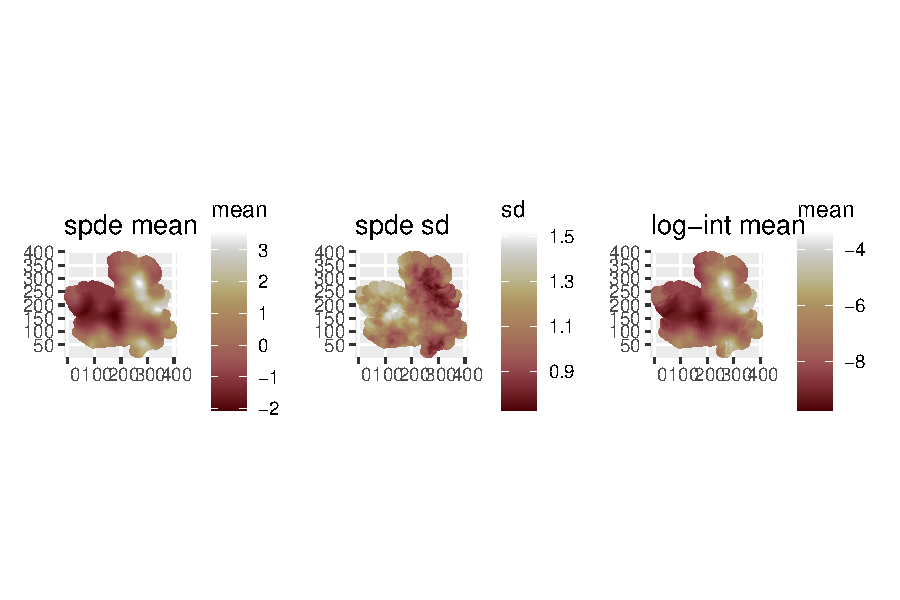
\includegraphics[keepaspectratio]{day3_practical_5_files/figure-pdf/unnamed-chunk-107-1.pdf}}
\end{center}

\begin{Shaded}
\begin{Highlighting}[]
\FunctionTok{ggplot}\NormalTok{(}\AttributeTok{data=}\NormalTok{preds}\SpecialCharTok{$}\NormalTok{log\_int) }\SpecialCharTok{+} 
  \FunctionTok{geom\_sf}\NormalTok{(}\FunctionTok{aes}\NormalTok{(}\AttributeTok{color =}\NormalTok{ sd)) }\SpecialCharTok{+}
  \FunctionTok{scale\_color\_scico}\NormalTok{() }\SpecialCharTok{+}
 \FunctionTok{ggtitle}\NormalTok{(}\StringTok{"log{-}int sd"}\NormalTok{) }\SpecialCharTok{+}
  \FunctionTok{plot\_layout}\NormalTok{(}\AttributeTok{ncol=}\DecValTok{2}\NormalTok{)}
\end{Highlighting}
\end{Shaded}

\begin{center}
\pandocbounded{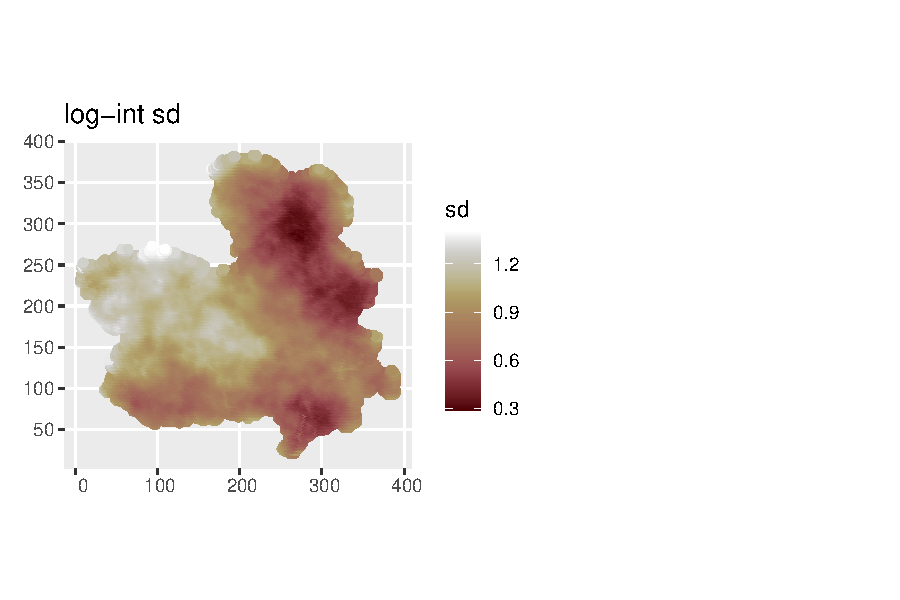
\includegraphics[keepaspectratio]{day3_practical_5_files/figure-pdf/unnamed-chunk-107-2.pdf}}
\end{center}

\end{tcolorbox}

Instead of just looking at the posterior mean and standard deviation, it
can be usefull to look at \texttt{simulated\ fields} from the posterior
distribution. This is because the mean field is, by definition, smoother
than any realization of the field. So looking at simulation can give us
a better idea of how the field might look like. We can do this using the
\emph{generate()} function:

\begin{Shaded}
\begin{Highlighting}[]
\NormalTok{sim\_fields }\OtherTok{=} \FunctionTok{generate}\NormalTok{(fit3, pxl, }\SpecialCharTok{\textasciitilde{}}\FunctionTok{data.frame}\NormalTok{(}\AttributeTok{spde =}\NormalTok{ space,}
                                       \AttributeTok{log\_int =}\NormalTok{ Intercept }\SpecialCharTok{+}\NormalTok{ space }\SpecialCharTok{+}\NormalTok{ elev),}
                     \AttributeTok{n.samples =} \DecValTok{4}\NormalTok{)}

\FunctionTok{cbind}\NormalTok{(pxl,}\FunctionTok{sapply}\NormalTok{(sim\_fields, }\ControlFlowTok{function}\NormalTok{(x) x}\SpecialCharTok{$}\NormalTok{spde)) }\SpecialCharTok{\%\textgreater{}\%}
  \FunctionTok{pivot\_longer}\NormalTok{(}\SpecialCharTok{{-}}\NormalTok{geometry) }\SpecialCharTok{\%\textgreater{}\%}
  \FunctionTok{ggplot}\NormalTok{() }\SpecialCharTok{+} \FunctionTok{geom\_sf}\NormalTok{(}\FunctionTok{aes}\NormalTok{(}\AttributeTok{color =}\NormalTok{ value)) }\SpecialCharTok{+} 
  \FunctionTok{facet\_wrap}\NormalTok{(.}\SpecialCharTok{\textasciitilde{}}\NormalTok{name) }\SpecialCharTok{+} \FunctionTok{scale\_color\_scico}\NormalTok{() }\SpecialCharTok{+}
  \FunctionTok{ggtitle}\NormalTok{(}\StringTok{"simulated spatial fields"}\NormalTok{)}
\end{Highlighting}
\end{Shaded}

\pandocbounded{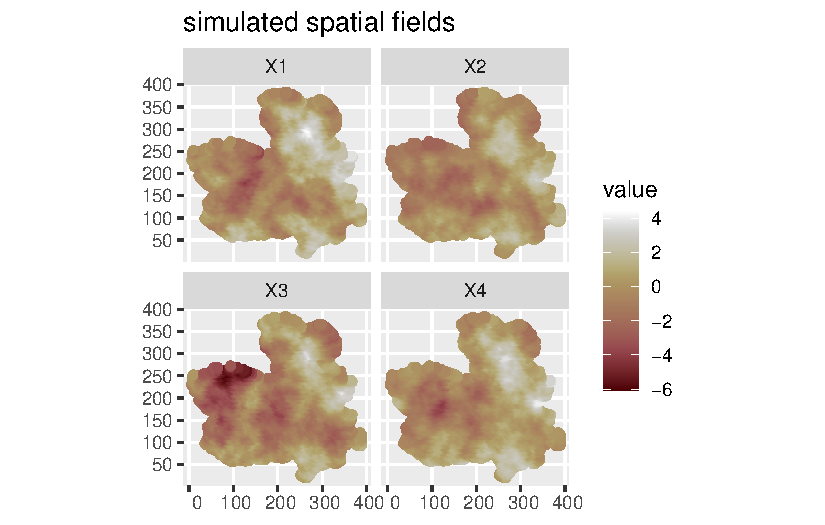
\includegraphics[keepaspectratio]{day3_practical_5_files/figure-pdf/unnamed-chunk-108-1.pdf}}

\begin{Shaded}
\begin{Highlighting}[]
\FunctionTok{cbind}\NormalTok{(pxl,}\FunctionTok{sapply}\NormalTok{(sim\_fields, }\ControlFlowTok{function}\NormalTok{(x) x}\SpecialCharTok{$}\NormalTok{log\_int)) }\SpecialCharTok{\%\textgreater{}\%}
  \FunctionTok{pivot\_longer}\NormalTok{(}\SpecialCharTok{{-}}\NormalTok{geometry) }\SpecialCharTok{\%\textgreater{}\%}
  \FunctionTok{ggplot}\NormalTok{() }\SpecialCharTok{+} \FunctionTok{geom\_sf}\NormalTok{(}\FunctionTok{aes}\NormalTok{(}\AttributeTok{color =}\NormalTok{ value)) }\SpecialCharTok{+} 
  \FunctionTok{facet\_wrap}\NormalTok{(.}\SpecialCharTok{\textasciitilde{}}\NormalTok{name) }\SpecialCharTok{+} \FunctionTok{scale\_color\_scico}\NormalTok{() }\SpecialCharTok{+} 
  \FunctionTok{ggtitle}\NormalTok{(}\StringTok{"simulated log intensity"}\NormalTok{)}
\end{Highlighting}
\end{Shaded}

\pandocbounded{\includegraphics[keepaspectratio]{day3_practical_5_files/figure-pdf/unnamed-chunk-108-2.pdf}}




\end{document}
